\documentclass[11pt]{article}

\usepackage[margin=1in]{geometry}
\usepackage{amsmath,amssymb,amsthm,mathtools}
\usepackage{booktabs}
\usepackage{enumitem}
\usepackage[hidelinks]{hyperref}
\usepackage{tikz}
\usepackage{pgfplots}
\pgfplotsset{compat=1.18}
\usetikzlibrary{arrows.meta,positioning,calc}

\theoremstyle{plain}
\newtheorem{theorem}{Theorem}[section]
\newtheorem{lemma}[theorem]{Lemma}
\newtheorem{proposition}[theorem]{Proposition}
\newtheorem{corollary}[theorem]{Corollary}
\theoremstyle{definition}
\newtheorem{definition}[theorem]{Definition}
\newtheorem{example}[theorem]{Example}
\newtheorem{protocol}[theorem]{Protocol}
\theoremstyle{remark}
\newtheorem{remark}[theorem]{Remark}
\newtheorem{conjecture}[theorem]{Conjecture}

\newcommand{\Q}{\mathbb{Q}}
\newcommand{\Z}{\mathbb{Z}}
\newcommand{\R}{\mathbb{R}}
\newcommand{\C}{\mathbb{C}}
\newcommand{\K}{K}
\newcommand{\OK}{\mathcal{O}_K}
\newcommand{\Tr}{\operatorname{Tr}}
\newcommand{\Nm}{\operatorname{N}}
\newcommand{\charpoly}{\operatorname{charpoly}}
\newcommand{\minpoly}{\operatorname{minpoly}}
\newcommand{\Mah}{\mathrm{M}}
\newcommand{\height}{\mathrm{H}}
\newcommand{\Fish}{\mathcal{I}}
\newcommand{\rr}{\mathbf{r}}
\newcommand{\xx}{\mathbf{x}}
\newcommand{\GG}{G}
\newcommand{\BB}{B}
\newcommand{\transpose}{^{\mathsf{T}}}
\newcommand{\inv}{^{-1}}
\DeclareMathOperator{\col}{col}
\DeclareMathOperator{\rank}{rank}
\DeclareMathOperator{\diag}{diag}
\DeclareMathOperator{\Cov}{Cov}
\DeclareMathOperator{\disc}{disc}

\title{\textbf{The Vector Substrate:\\ Number Fields as Exact Learning Geometry}}
\author{L00M Vector Substrate Project}
\date{June 2026}

\begin{document}
\maketitle

\begin{abstract}
We develop a framework in which a number field $\K=\Q(\theta)$ is treated \emph{simultaneously} as a
$\Q$--vector space, as a commutative matrix algebra (its regular representation, with multiplication by
$\theta$ realised by the companion matrix of the minimal polynomial), and as a Euclidean lattice (its
Minkowski embedding). The trace form $T(x,y)=\Tr_{\K/\Q}(xy)$ supplies a single, exact, rational metric
$\GG$ that unifies these three faces. We build an exact, fully reproducible \emph{learning} apparatus on
this geometry: an observation is captured precisely when its $\GG$--orthogonal residual against a forced
basis vanishes, and learning is the gated, witnessed growth of that basis by adjoining algebraic--integer
seeds and, when required, by passing to a disjoint compositum (whose Gram matrix is the Kronecker product
of the factor Grams). Model complexity is controlled by arithmetic height: the Mahler measure
$\Mah(\theta)=\height(\theta)^{\deg\theta}$, Landau's inequality, and Northcott finiteness yield an
exact-integer admissibility gate. Our information--geometric reading \emph{assembles classical facts}: the
trace form is the Gram of the Minkowski embedding ($\GG=M\transpose M$, $\det\GG=d_\K$), and the Fisher
information of a Gaussian location family $\mathcal N(Ma,I)$ is $M\transpose M$. From these we read the trace
form as the Fisher metric of two natural models, pin the model--dependent conformal constant ($c=1$ for the
Gaussian, $c=n$ for the maximum--entropy family on the Galois conjugates), and obtain a
residual--norm--as--information--distance reading for the learner: on the trace--zero (residual) subspace
$\lVert\rr\rVert_{\GG}^2=n\cdot\Fish(\rr)$. We do not claim to settle an open problem---the contribution is
this synthesis and its use. We then derive an information gain--versus--cost growth threshold whose floor is
provably nonzero for non--reciprocal seeds (Smyth's theorem) and discuss the reciprocal case (Lehmer's
conjecture). Two further bridges tighten the picture: the regular representation is
diagonalised by the Minkowski embedding, so its spectrum \emph{is} the set of Galois conjugates and the
Mahler measure is a spectral invariant of the companion matrix; and the Jeffreys volume of the Fisher
metric equals $\sqrt{\det\GG}=\sqrt{|d_\K|}$ (in an integral basis), identifying the field discriminant with
an information volume.
Throughout we separate \emph{provable} statements (with proofs or exact computations) from \emph{conjectural}
or model--dependent ones; every numerical claim is matched to a machine--checked verification probe, and a
notation key and an honesty ledger make the provable/conjectural split scannable.
\end{abstract}

\tableofcontents

\section{Introduction and thesis}\label{sec:intro}

\subsection*{The thesis}
Let $\K=\Q(\theta)$ be a number field of degree $n=[\K:\Q]$, and let $m_\theta\in\Z[x]$ be the minimal
polynomial of $\theta$. The field $\K$ admits three classical descriptions:
\begin{enumerate}[label=(\roman*)]
  \item a $\Q$--vector space of dimension $n$, with basis $\{1,\theta,\dots,\theta^{n-1}\}$;
  \item a commutative subalgebra of $M_n(\Q)$, via the \emph{regular representation}
        $\rho\colon \K\to M_n(\Q)$, $x\mapsto(\text{multiplication by }x)$, under which $\rho(\theta)$ is
        the companion matrix $C(m_\theta)$;
  \item a full--rank Euclidean lattice in $\R^n$, via the Minkowski embedding
        $\sigma=(\sigma_1,\dots,\sigma_n)$ of the $n$ archimedean places.
\end{enumerate}
These are not three analogies but \emph{one object viewed in three coordinate systems}, glued by a single
rational bilinear form: the trace form
\begin{equation}\label{eq:traceform}
  T(x,y) \;=\; \Tr_{\K/\Q}(xy) \;=\; \sum_{i=1}^{n}\sigma_i(x)\,\sigma_i(y).
\end{equation}
The matrix $\GG=\big(\Tr(\omega_i\omega_j)\big)_{ij}$ of $T$ in a basis $\{\omega_i\}$ is the bridge: it is
the Gram matrix of the algebra's pairing, and simultaneously the Gram matrix of the embedded lattice.

\subsection*{Why this matters for learning}
Equation~\eqref{eq:traceform} makes $\K$ a metric space in which membership is decidable by exact rational
arithmetic. Fix a ``forced'' subspace spanned by a small dictionary of algebraic--integer seeds. An
observation $\xx\in\K$ is \emph{captured} exactly when its $\GG$--orthogonal residual $\rr=\xx-P\xx$ is
zero, where $P$ is the trace--form projector onto the dictionary. Capture is decided over $\Q$; only its
\emph{magnitude} $\lVert\rr\rVert_{\GG}$ is ever read as a real number. ``Understanding'' is, in this
framework, exactly a zero residual; \emph{learning} is the disciplined enlargement of the dictionary so as
to capture persistent residuals.

\subsection*{Contributions}
\begin{enumerate}[label=(C\arabic*),leftmargin=*]
  \item \textbf{An exact trace--form learning geometry} (\S\ref{sec:geometry}--\ref{sec:learning}): the
        projector/residual calculus over $\Q$, a propose--for--confirm growth protocol with a tamper--evident
        witness chain, and an exact \emph{coordinates--to--minimal--polynomial} bridge computed as the
        largest invariant factor of $xI-\rho(\alpha)$ via Smith normal form.
  \item \textbf{Cross--field growth} (\S\ref{subsec:compositum}): when a residual lies outside the current
        field, the model grows to a disjoint compositum, whose trace--form Gram is the Kronecker product
        $\GG_{\K\!L}=\GG_\K\otimes\GG_L$ (Proposition~\ref{prop:kron}); the non--disjoint case is isolated and
        flagged open.
  \item \textbf{Height--based capacity control} (\S\ref{sec:capacity}): an exact--integer admissibility gate
        founded on $\Mah(\theta)=\height(\theta)^{\deg\theta}$, Landau's inequality, and Northcott finiteness,
        with a provable separation between the exact decision boundary and float--valued display quantities.
  \item \textbf{Information geometry (a synthesis)} (\S\ref{sec:infogeo}): the classical facts
        $\GG=M\transpose M$ and $\Fish_{\mathrm{Gauss}}=M\transpose M$ make the trace form a Fisher metric; we
        pin the conformal constant ($c=1$ Gaussian vs $c=n$ max--entropy) and show
        $\lVert\rr\rVert_{\GG}^2=n\,\Fish(\rr)$ on the residual subspace
        (Theorems~\ref{thm:gaussfisher}--\ref{thm:resfisher}).
  \item \textbf{Two structural bridges} (\S\ref{subsec:spectral}, \S\ref{sec:infogeo}): the regular
        representation is diagonalised by the Minkowski embedding, so its spectrum is the set of Galois
        conjugates and the Mahler measure is a spectral invariant of the companion matrix
        (Proposition~\ref{prop:spectral}, Remark~\ref{rem:mahlerspectral}); and the Jeffreys volume of the
        Fisher metric is $\sqrt{\det\GG}=\sqrt{|d_\K|}$ (in an integral basis), identifying the field
        discriminant with an information volume (Proposition~\ref{prop:discvol}).
  \item \textbf{A growth threshold} (\S\ref{sec:threshold}): an information gain--versus--cost criterion
        with a \emph{provable} nonzero floor from Smyth's theorem, and a precise accounting of what is proved
        versus conjectured.
  \item \textbf{Applications} (\S\ref{sec:apps}): streaming anomaly/novelty detection, a capacity--bounded
        dictionary learner, and the natural--gradient and minimum--description--length readings of the above.
\end{enumerate}

\paragraph{Honesty discipline.} We use \emph{Theorem}/\emph{Proposition}/\emph{Lemma} only for statements we
prove or verify by exact computation, and \emph{Conjecture}/\emph{Remark} for model--dependent or heuristic
claims (the choice of statistical model, the information exchange rate, the effective Mahler floor, the
complex--embedding normalisation). Every displayed numerical value is reproduced by a machine--checked probe
(Appendix~\ref{sec:appendix}).

\paragraph{Related work and positioning.} The ingredients are classical. The trace form, Minkowski embedding,
different, and discriminant are standard \cite{Neukirch,Marcus}; invariant factors and the rational canonical
form are textbook linear algebra \cite{DummitFoote}; Mahler measure, Northcott's theorem, and the Lehmer and
Smyth bounds are staples of height theory \cite{Mahler,Northcott,Lehmer,Smyth,BombieriGubler}; and the
Fisher--information and natural--gradient viewpoint is Amari's \cite{Amari,AmariNagaoka}. The contribution is
not a new theorem in any of these areas but their \emph{assembly} into an exact, additive learning geometry:
a model whose state is a basis of a number field, whose loss is a trace--form residual decided over $\Q$, and
whose capacity is bounded by arithmetic height. The trace form plays here the role a kernel plays in kernel
methods---a fixed positive form in which all inner products are taken---but it is exact, integer--valued, and
carries arithmetic (the discriminant, the different, the height floor) that an analytic kernel does not.

\begin{figure}[ht]
\centering
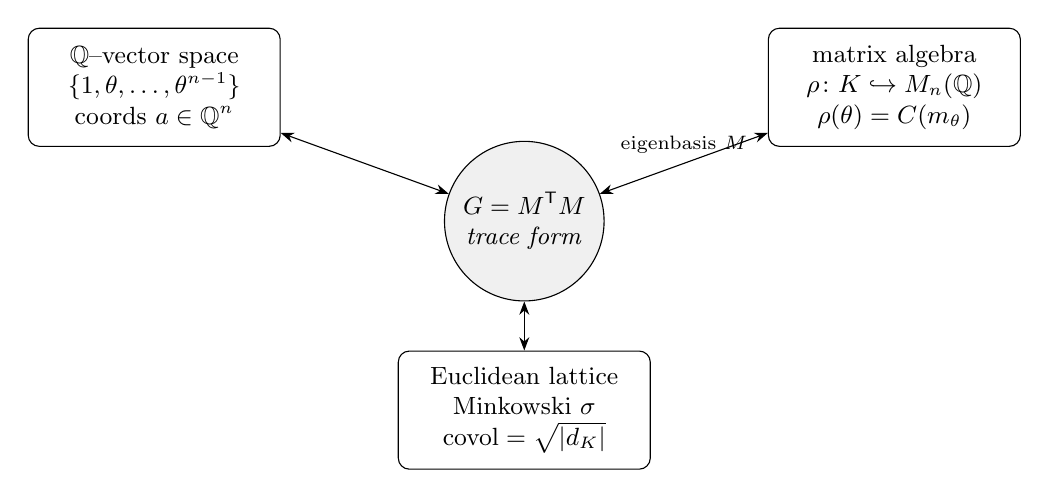
\begin{tikzpicture}[
  view/.style={draw, rounded corners, align=center, minimum width=3.2cm, minimum height=1.5cm, font=\small},
  glue/.style={draw, circle, align=center, font=\small, minimum size=1.7cm, fill=black!6},
  >={Stealth[]}]
  \node[view] (vs) at (-4.7,1.7) {$\Q$--vector space\\$\{1,\theta,\dots,\theta^{n-1}\}$\\coords $a\in\Q^n$};
  \node[view] (ma) at (4.7,1.7) {matrix algebra\\$\rho\colon\K\hookrightarrow M_n(\Q)$\\$\rho(\theta)=C(m_\theta)$};
  \node[view] (la) at (0,-2.4) {Euclidean lattice\\Minkowski $\sigma$\\$\operatorname{covol}=\sqrt{|d_\K|}$};
  \node[glue] (g) at (0,0) {$\GG=M\transpose M$\\\emph{trace form}};
  \draw[<->] (vs) -- (g);
  \draw[<->] (ma) -- (g) node[midway,above,font=\scriptsize] {eigenbasis $M$};
  \draw[<->] (la) -- (g);
\end{tikzpicture}
\caption{Three views of $\K=\Q(\theta)$, glued by the single trace--form Gram $\GG$: a $\Q$--vector space of
coordinates, a commutative matrix algebra (the regular representation $\rho$, diagonalised by the embedding
matrix $M$, Proposition~\ref{prop:spectral}), and a Euclidean lattice (the Minkowski embedding $\sigma$,
covolume $\sqrt{|d_\K|}$). The same exact rational matrix $\GG$ serves all three.}
\label{fig:triptych}
\end{figure}

\begin{table}[ht]
\centering
\small
\begin{tabular}{ll}
\toprule
Symbol & Meaning \\
\midrule
$\K=\Q(\theta)$, $n$ & number field of degree $n=[\K:\Q]$ with generator $\theta$ \\
$(r_1,r_2)$ & numbers of real / complex--conjugate embeddings, $n=r_1+2r_2$ \\
$\OK$, $d_\K$ & ring of integers; field discriminant \\
$m_\theta$, $C(m_\theta)$ & minimal polynomial of $\theta$; its companion matrix \\
$\rho$ & regular representation $\K\hookrightarrow M_n(\Q)$, $\rho(\theta)=C(m_\theta)$ \\
$\sigma_k$, $M$ & the $n$ embeddings $\K\to\C$; embedding matrix $M_{ki}=\sigma_k(\omega_i)$ \\
$\GG$, $T$ & trace--form Gram $\GG_{ij}=\Tr(\omega_i\omega_j)=M\transpose M$; $T(x,y)=\Tr(xy)$ \\
$\BB$, $\col\BB$ & forced basis (the model state); its column span \\
$P$, $\rr$ & trace--form projector onto $\col\BB$; residual $\rr=\xx-P\xx$ \\
$\Mah(\theta)$, $\height(\theta)$ & Mahler measure $\Mah=\height^{\deg}$; absolute height \\
$\mu_S$, $\mu_L$ & Smyth floor $1.3247\ldots$ (theorem); Lehmer value $1.17628\ldots$ (conjectural) \\
$\Fish$, $\lambda$ & Fisher information; information exchange rate (cost of one parameter) \\
\bottomrule
\end{tabular}
\caption{Notation used throughout.}
\label{tab:notation}
\end{table}

\section{Preliminaries}\label{sec:prelim}

\subsection{Number fields and the regular representation}
Let $\K=\Q(\theta)$ with $m_\theta(x)=x^n+c_{n-1}x^{n-1}+\dots+c_0\in\Z[x]$ irreducible. Write
$\OK$ for the ring of integers. For $x\in\K$, multiplication by $x$ is a $\Q$--linear endomorphism of $\K$;
in the power basis $\{1,\theta,\dots,\theta^{n-1}\}$ it is a matrix $\rho(x)\in M_n(\Q)$.

\begin{proposition}[Regular representation]\label{prop:regrep}
The map $\rho\colon\K\to M_n(\Q)$ is an injective $\Q$--algebra homomorphism, and $\rho(\theta)=C(m_\theta)$,
the companion matrix of $m_\theta$. For $x\in\K$ with minimal polynomial $m_x$ of degree $d\mid n$, the
characteristic and minimal polynomials of the matrix $\rho(x)$ are
\begin{equation}\label{eq:charmin}
  \charpoly(\rho(x)) = m_x^{\,n/d}, \qquad \minpoly(\rho(x)) = m_x .
\end{equation}
\end{proposition}
\begin{proof}
$\rho$ is a ring homomorphism because multiplication in $\K$ is associative and bilinear; it is injective
because $\rho(x)=0$ forces $x\cdot 1=0$, i.e. $x=0$. The matrix of multiplication by $\theta$ sends
$\theta^{k}\mapsto\theta^{k+1}$ for $k<n-1$ and $\theta^{n-1}\mapsto -\sum_{j<n}c_j\theta^{j}$, which is
exactly $C(m_\theta)$. For~\eqref{eq:charmin}: $\K$ is a vector space over the subfield $\Q(x)$ of degree
$n/d$, and as a $\Q(x)$--module $\K\cong \Q(x)^{n/d}$. Multiplication by $x$ acts on each $\Q(x)$--summand as
multiplication by $x$, whose matrix over $\Q$ is $C(m_x)$. Hence $\rho(x)$ is similar over $\Q$ to a direct
sum of $n/d$ copies of $C(m_x)$, giving $\charpoly(\rho(x))=m_x^{n/d}$ and $\minpoly(\rho(x))=m_x$ (the
minimal polynomial of a block--diagonal matrix is the least common multiple of the blocks' minimal
polynomials, here all equal to $m_x$).
\end{proof}

\begin{example}[The regular representation of $\varphi$]\label{ex:regrep}
For $\varphi$ with $m_\varphi=x^2-x-1$ we have
$\rho(\varphi)=C(m_\varphi)=\left(\begin{smallmatrix}0&1\\1&1\end{smallmatrix}\right)$, and the field trace and
norm appear as matrix invariants: $\Tr\rho(\varphi)=1=\Tr_{\K/\Q}(\varphi)$ and
$\det\rho(\varphi)=-1=\mathrm N_{\K/\Q}(\varphi)$. For $\alpha=\sqrt5=2\varphi-1$,
$\rho(\alpha)=2\rho(\varphi)-I=\left(\begin{smallmatrix}-1&2\\2&1\end{smallmatrix}\right)$ has
$\charpoly=\minpoly=x^2-5$. For the rational $\alpha=3$, $\rho(3)=3I$ is derogatory: $\charpoly=(x-3)^2$ but
$\minpoly=x-3$---the multiplicity $n/d=2$ of~\eqref{eq:charmin} made visible.
\end{example}

\subsection{Spectral picture: the regular representation is the conjugates}\label{subsec:spectral}
\begin{proposition}[Spectral unification]\label{prop:spectral}
For every $x\in\K$ the eigenvalues of $\rho(x)$ are exactly the $n$ conjugates
$\sigma_1(x),\dots,\sigma_n(x)$, and the embedding matrix $M$ diagonalises the regular representation:
\begin{equation}\label{eq:diag}
  M\,\rho(x)\,M\inv=\diag\big(\sigma_1(x),\dots,\sigma_n(x)\big)\qquad\text{for all }x\in\K.
\end{equation}
The matrix--algebra and lattice views are thus one operator in two bases: $\rho(x)$ in the power basis,
$\diag(\sigma_k(x))$ in the eigenbasis supplied by $M$.
\end{proposition}
\begin{proof}
For $x\in\K$ and a basis element $\omega_j$, $x\omega_j=\sum_i\rho(x)_{ij}\omega_i$; applying the embedding
$\sigma_k$ (a ring homomorphism) gives $\sigma_k(x)\sigma_k(\omega_j)=\sum_i\rho(x)_{ij}\sigma_k(\omega_i)$,
that is $\sigma_k(x)M_{kj}=\sum_i M_{ki}\rho(x)_{ij}=(M\rho(x))_{kj}$. Hence $M\rho(x)=\diag(\sigma_k(x))\,M$,
and $M$ is invertible since $\det\GG=(\det M)^2=d_\K\neq0$ (Theorem~\ref{thm:GMM}). Rearranging
gives~\eqref{eq:diag}, so the eigenvalues of $\rho(x)$ are the diagonal entries $\sigma_k(x)$; equivalently
$\charpoly(\rho(x))=\prod_k(T-\sigma_k(x))$, the field polynomial of $x$.
\end{proof}

\begin{remark}[Mahler measure is a spectral invariant]\label{rem:mahlerspectral}
For an algebraic integer $\theta$ generating $\K$, $\rho(\theta)=C(m_\theta)$ and~\eqref{eq:diag} identify
the spectrum of $\rho(\theta)$ with the conjugates $\{\sigma_k(\theta)\}$, the roots of $m_\theta$. Hence the
Mahler measure is read off the spectrum,
\begin{equation}\label{eq:mahlerspectral}
  \Mah(\theta)=\!\!\prod_{\lambda\in\operatorname{spec}\rho(\theta),\;|\lambda|>1}\!\!|\lambda|,
\end{equation}
the product of the companion eigenvalues outside the unit circle. Equivalently, by Jensen's formula
\cite{Mahler}, $\Mah(\theta)=\exp\!\int_0^1\log\bigl|m_\theta(e^{2\pi i t})\bigr|\,dt$. For
$\theta=\sqrt2+\sqrt3$ the spectrum is $\{\pm\sqrt2\pm\sqrt3\}$ and $\Mah(\theta)=(\sqrt2+\sqrt3)^2=5+2\sqrt6$;
for the plastic number (Smyth's minimiser, the real root of $x^3-x-1$) only the real eigenvalue exceeds $1$,
so $\Mah=\mu_S=1.3247\ldots$ (Figure~\ref{fig:mahler}).
\end{remark}

\begin{proposition}[Height as dynamical entropy {\cite{Yuzvinskii,LSW}}]\label{prop:lsw}
The companion matrix $C(m_\theta)\in M_n(\Z)$ defines an endomorphism of the torus $\R^n/\Z^n$, whose
topological entropy equals $\log\Mah(\theta)$. For a single endomorphism this is the classical
Yuzvinskii--Bowen identity \cite{Yuzvinskii}; the Lind--Schmidt--Ward theorem \cite{LSW} is its $\Z^d$
generalisation, specialising to the present $d=1$ case. The description length $\log\Mah$ that prices growth
in \S\ref{sec:threshold} is therefore the entropy of the toral map generated by $\rho(\theta)$---tying the
matrix view (\S\ref{subsec:spectral}), the height view (\S\ref{sec:capacity}), and the threshold
(\S\ref{sec:threshold}) to one invariant.
\end{proposition}

\begin{example}[Diagonalising $\rho$ in $\Q(\sqrt5)$]\label{ex:spectral}
For $\K=\Q(\sqrt5)$, $\rho(\varphi)=C(x^2-x-1)=\left(\begin{smallmatrix}0&1\\1&1\end{smallmatrix}\right)$ and
$M=\left(\begin{smallmatrix}1&\varphi\\1&\varphi'\end{smallmatrix}\right)$ (rows the two embeddings, $\varphi'=\tfrac{1-\sqrt5}2$). Then
\[
  M\,\rho(\varphi)\,M\inv=\diag(\varphi,\varphi')=\diag\!\Big(\tfrac{1+\sqrt5}2,\ \tfrac{1-\sqrt5}2\Big),
\]
so the eigenvalues of the companion matrix are exactly the two conjugates and
$\charpoly(\rho(\varphi))=x^2-x-1=m_\varphi$. The same $M$ diagonalises $\rho(x)$ for \emph{every}
$x\in\Q(\sqrt5)$ at once (Proposition~\ref{prop:spectral}), and the trace form is the Gram of these
eigen--coordinates, $\GG=M\transpose M$.
\end{example}

\begin{example}[The spectrum of $\rho(\sqrt2+\sqrt3)$]\label{ex:spectral4}
For $\theta=\sqrt2+\sqrt3$, the matrix $\rho(\theta)=C(x^4-10x^2+1)$ is $4\times4$ with
$\charpoly(\rho(\theta))=x^4-10x^2+1=m_\theta$ and eigenvalues the four conjugates
$\{\pm\sqrt2\pm\sqrt3\}\approx\{\pm3.146,\ \pm0.318\}$. Two lie outside the unit circle, so
by~\eqref{eq:mahlerspectral} $\Mah(\theta)=(\sqrt2+\sqrt3)^2=5+2\sqrt6\approx9.899$; equivalently $\log\Mah$
is the topological entropy of the toral endomorphism of $C(x^4-10x^2+1)$ (Proposition~\ref{prop:lsw}). All
values are probe--checked.
\end{example}

\subsection{Invariant factors and Smith normal form}
The rational canonical form refines~\eqref{eq:charmin}. For $A\in M_n(\Q)$ the \emph{invariant factors} are
the monic polynomials $f_1\mid f_2\mid\dots\mid f_k$ obtained from the Smith normal form of the
characteristic matrix $xI-A$ over the principal ideal domain $\Q[x]$; they satisfy $\prod_i f_i=\charpoly(A)$
and $f_k=\minpoly(A)$, and they form a \emph{complete} invariant for similarity over $\Q$. We will use:

\begin{corollary}\label{cor:largestif}
For $\alpha\in\K=\Q(\theta)$, the minimal polynomial $m_\alpha$ equals the largest invariant factor of
$xI-\rho(\alpha)$.
\end{corollary}
\begin{proof}
Immediate from $f_k=\minpoly(\rho(\alpha))=m_\alpha$ by Proposition~\ref{prop:regrep}.
\end{proof}
\begin{theorem}[Completeness of invariant factors]\label{thm:ifcomplete}
Matrices $A,A'\in M_n(\Q)$ are similar over $\Q$ if and only if they have the same invariant factors. The
characteristic polynomial alone is a complete similarity invariant only on the non--derogatory locus (where
$\charpoly=\minpoly$); in general it is not.
\end{theorem}
\begin{proof}
$A\sim A'$ over $\Q$ iff the $\Q[x]$--modules $\Q[x]^n/(xI-A)$ and $\Q[x]^n/(xI-A')$ are isomorphic, iff
$xI-A$ and $xI-A'$ have the same Smith normal form, i.e. the same invariant factors; this is the structure
theorem for finitely generated modules over the PID $\Q[x]$ \cite[Ch.~12]{DummitFoote}. The non--derogatory
case is $k=1$, where the single invariant factor equals the characteristic polynomial.
\end{proof}

\begin{example}[Characteristic polynomial is insufficient]\label{ex:phiphi}
In $\K=\Q(\varphi)$ compare the block sum $\rho(\varphi)\oplus\rho(\varphi)=C(m_\varphi)\oplus C(m_\varphi)$
with the companion $C\big((x^2-x-1)^2\big)$ of $(x^2-x-1)^2=x^4-2x^3-x^2+2x+1$. Both are $4\times4$ with
characteristic polynomial $(x^2-x-1)^2$ and trace $2$, yet they are \emph{not} similar: the former has
minimal polynomial $x^2-x-1$ and invariant factors $(x^2-x-1,\,x^2-x-1)$, the latter the single invariant
factor $(x^2-x-1)^2$. The largest invariant factor separates them; the characteristic polynomial does not.
This is precisely why Theorem~\ref{thm:bridge} reads the minimal polynomial as the largest invariant factor.
\end{example}

\begin{remark}[Computing the Smith normal form]\label{rem:snf}
Over the Euclidean domain $\Q[x]$ the invariant factors are obtained from $xI-A$ by the standard reduction:
repeatedly select a nonzero entry of least degree as pivot, clear its row and column by polynomial division
(re--pivoting whenever a smaller--degree remainder surfaces), and then enforce divisibility of the trailing
submatrix; the resulting monic diagonal entries of degree $\ge1$ are $f_1\mid\dots\mid f_k$. The procedure is
exact over $\Q$ and terminates because the minimal pivot degree strictly decreases.
\end{remark}

\begin{example}[Why the full list is needed]\label{ex:jordan}
Even the pair $(\charpoly,\minpoly)$ is incomplete once an invariant factor has multiplicity $\ge3$. With
$J_2=\left(\begin{smallmatrix}0&1\\0&0\end{smallmatrix}\right)$ and $J_1=(0)$, the matrices $J_2\oplus J_2$ and
$J_2\oplus J_1\oplus J_1$ both have characteristic polynomial $x^4$ and minimal polynomial $x^2$, yet they are
\emph{not} similar: their invariant factors are $(x^2,x^2)$ and $(x,x,x^2)$. Only the full invariant--factor
list separates them---one reason the bridge (Theorem~\ref{thm:bridge}) reads the largest invariant factor from
the Smith normal form rather than from the characteristic polynomial.
\end{example}

This is the exact algorithm underlying our coordinates--to--minimal--polynomial bridge
(\S\ref{subsec:bridge}); it is purely rational and never computes a root.

\subsection{The Minkowski embedding and the trace form}
Let $\sigma_1,\dots,\sigma_{r_1}\colon\K\to\R$ be the real embeddings and
$\sigma_{r_1+1},\bar\sigma_{r_1+1},\dots$ the complex pairs, $n=r_1+2r_2$. The Minkowski embedding is
$\sigma(x)=(\sigma_1(x),\dots,\sigma_n(x))$. The trace is the sum of conjugates,
$\Tr_{\K/\Q}(x)=\sum_i\sigma_i(x)$, whence~\eqref{eq:traceform}. In a basis $\{\omega_i\}$ define the Gram
matrix and the embedding matrix
\begin{equation}\label{eq:GandM}
  \GG_{ij}=\Tr(\omega_i\omega_j), \qquad M_{ki}=\sigma_k(\omega_i)\in\C.
\end{equation}

\begin{theorem}[Trace form as embedding Gram]\label{thm:GMM}
$\GG = M\transpose M$. In particular, if $\K$ is totally real ($r_2=0$) then $M$ is real and $\GG$ is a
genuine Gram matrix of $n$ vectors in $\R^n$. For an integral basis of $\OK$, $\det\GG=\disc(\K)=d_\K$; for
a sub--order $\Lambda\subseteq\OK$, $\det\GG=[\OK:\Lambda]^2\,d_\K$. The covolume of the Minkowski lattice is
treated in \S\ref{subsec:lattice}.
\end{theorem}
\begin{proof}
$\GG_{ij}=\Tr(\omega_i\omega_j)=\sum_k\sigma_k(\omega_i\omega_j)=\sum_k\sigma_k(\omega_i)\sigma_k(\omega_j)
=\sum_k M_{ki}M_{kj}=(M\transpose M)_{ij}$, using that each $\sigma_k$ is a ring homomorphism. The
discriminant identity $\det\GG=d_\K$ for an integral basis and the index correction are standard
\cite{Neukirch,Marcus}; the relation $\det\GG=(\det M)^2$ yields the lattice covolume of
\S\ref{subsec:lattice}.
\end{proof}

\begin{remark}[Signature and totally real fields]\label{rem:signature}
For $r_2>0$ the real quadratic form $\sum_i\sigma_i(x)^2$ has signature $(r_1+r_2,r_2)$; the
positive--definite companion is the Hermitian trace form of \S\ref{subsec:complex}. Apart from that
subsection's Gaussian--integer example, all worked examples here are totally real, where $\GG=M\transpose M$
is itself positive definite and no normalisation subtlety arises.
\end{remark}

\begin{example}[The golden field]\label{ex:golden}
Let $\K=\Q(\sqrt5)=\Q(\varphi)$, $\varphi=\tfrac{1+\sqrt5}2$, $m_\varphi=x^2-x-1$, so $\rho(\varphi)
=\left(\begin{smallmatrix}0&1\\1&1\end{smallmatrix}\right)$. The embeddings send $\varphi\mapsto\varphi$ and
$\varphi\mapsto\varphi'=\tfrac{1-\sqrt5}2$, so in the basis $\{1,\varphi\}$,
\[
  M=\begin{pmatrix}1&\varphi\\ 1&\varphi'\end{pmatrix},\qquad
  \GG=M\transpose M=\begin{pmatrix}2&1\\1&3\end{pmatrix},\qquad
  \det\GG=5=d_{\Q(\sqrt5)} .
\]
Here $\Tr(1)=2$, $\Tr(\varphi)=\varphi+\varphi'=1$, $\Tr(\varphi^2)=\varphi^2+\varphi'^2=3$, and
$\{1,\varphi\}$ is an integral basis ($\Z[\varphi]=\OK$).
\end{example}

\begin{example}[A biquadratic field]\label{ex:biquad}
Let $\K=\Q(\sqrt2,\sqrt3)$ with the product basis $\{1,\sqrt2,\sqrt3,\sqrt6\}$. The four embeddings send
$(\sqrt2,\sqrt3)\mapsto(\pm\sqrt2,\pm\sqrt3)$ (four sign choices), and
\[
  \GG=\diag(4,8,12,24),\qquad \det\GG = 9216 = 2^{10}3^2 .
\]
Since $d_{\Q(\sqrt2,\sqrt3)}=2304=2^8 3^2$, this basis spans a sub--order of index
$[\OK:\Lambda]=\sqrt{9216/2304}=2$; the Gram and all geometry below are taken relative to this convenient
basis.
\end{example}

\subsection{Complex embeddings and the positive--definite form}\label{subsec:complex}
When $r_2>0$ the trace form $T(x,y)=\sum_i\sigma_i(x)\sigma_i(y)$ is \emph{indefinite}: a complex place
contributes, through its conjugate pair $\sigma,\bar\sigma$, the term
$\sigma(x)\sigma(y)+\bar\sigma(x)\bar\sigma(y)=2\Re\big(\sigma(x)\sigma(y)\big)$, a hyperbolic plane, and the
signature of $T$ is $(r_1+r_2,\,r_2)$. The positive--definite companion is the \emph{Hermitian trace form}
\begin{equation}\label{eq:T2}
  T_2(x,y)=\sum_{i=1}^n\sigma_i(x)\overline{\sigma_i(y)}
  =\sum_{i\le r_1}\sigma_i(x)\sigma_i(y)
   +2\sum_{j=1}^{r_2}\Re\big(\sigma_{r_1+j}(x)\overline{\sigma_{r_1+j}(y)}\big),
\end{equation}
the pullback of the canonical (Minkowski) inner product on $\R^{r_1}\times\C^{r_2}\cong\R^n$. Its Gram matrix
is $G_2=M^{*}M$ ($M^{*}$ the conjugate transpose), positive definite, with $\det G_2=|d_\K|$ for an integral
basis, so the Minkowski lattice has covolume $\sqrt{\det G_2}=\sqrt{|d_\K|}$ in this metric (the geometric
embedding $\C\cong\R^2$ rescales the complex coordinates to the textbook value $2^{-r_2}\sqrt{|d_\K|}$). For
totally real fields $r_2=0$ and $T_2=T$,
$G_2=\GG=M\transpose M$ (Theorem~\ref{thm:GMM}); all of \S\ref{sec:geometry}--\ref{sec:infogeo} is written for
$\GG$ and applies verbatim to $G_2$ in the complex case, with $M\transpose$ replaced by $M^{*}$ and the
isotropic Gaussian of \S\ref{sec:infogeo} taken on the canonical real space $\R^n$ with metric $G_2$.

\begin{example}[The Gaussian field]\label{ex:gaussint}
$\K=\Q(i)$ ($r_1=0$, $r_2=1$, $n=2$), basis $\{1,i\}$, embeddings $i\mapsto i$ and $i\mapsto-i$. The trace
form is
\[
  \GG=\begin{pmatrix}\Tr(1)&\Tr(i)\\\Tr(i)&\Tr(i^2)\end{pmatrix}=\begin{pmatrix}2&0\\0&-2\end{pmatrix},
\]
indefinite of signature $(1,1)$, while the Hermitian form~\eqref{eq:T2} is
$G_2=\left(\begin{smallmatrix}2&0\\0&2\end{smallmatrix}\right)=2I$, positive definite, with $\det G_2=4=|d_{\Q(i)}|$
so the covolume in this metric is $\sqrt4=2=\sqrt{|d_\K|}$; the geometric rescaling returns the
unit--covolume Gaussian lattice $\Z[i]$ ($2^{-1}\sqrt4=1$). Membership and residual are taken with respect to
$G_2$.
\end{example}

\begin{example}[A cubic with a complex place]\label{ex:cubic2}
$\K=\Q(\sqrt[3]2)$ has $r_1=1,r_2=1,n=3$; the embeddings send $\sqrt[3]2$ to the real $\sqrt[3]2$ and to the
complex pair $\sqrt[3]2\,\omega,\sqrt[3]2\,\omega^2$ ($\omega=e^{2\pi i/3}$). On the power basis
$\{1,\sqrt[3]2,\sqrt[3]4\}$, using $\Tr(1)=3$ and $\Tr(\sqrt[3]2)=\Tr(\sqrt[3]4)=0$,
\[
  \GG=\begin{pmatrix}3&0&0\\0&0&6\\0&6&0\end{pmatrix},\qquad \det\GG=-108=d_{\Q(\sqrt[3]2)} .
\]
This $\GG$ is \emph{indefinite}, of signature $(2,1)=(r_1+r_2,r_2)$ (eigenvalues $3,\pm6$), exactly as
above; the positive--definite companion is the Hermitian $G_2=M^{*}M$. The exact identity $\det\GG=d_\K$
persists through the complex place.
\end{example}

\subsection{The Minkowski lattice}\label{subsec:lattice}
By Theorem~\ref{thm:GMM} the embedding $\sigma$ sends $\OK$ to a full--rank lattice
$\Lambda_\K=\sigma(\OK)\subset\R^n$ with Gram matrix $\GG$. Its covolume is
$\operatorname{covol}(\Lambda_\K)=\sqrt{\det\GG}=\sqrt{|d_\K|}$ ($=\sqrt{d_\K}$ for a totally real field; the
geometric normalisation of the complex places gives $2^{-r_2}\sqrt{|d_\K|}$ instead, \S\ref{subsec:complex}).
For $\Q(\sqrt5)$, $\det\GG=5$ and the covolume is $\sqrt5$. Lattice and algebra thus share a
single matrix $\GG$: distances, volumes, and the trace pairing are all computed by the same exact rational
form, and the ``forced'' directions of the learner (\S\ref{sec:learning}) are a sublattice spanned by a
chosen basis.

\begin{remark}[The lattice meets the height floor]\label{rem:lehmerlattice}
The Mahler measure that gates capacity (\S\ref{sec:capacity}) is a function of where the conjugates of
$\theta$ sit, hence of the geometry of $\Lambda_\K$. Lehmer's problem---whether $\Mah(\theta)\ge\mu_L>1$ for
some universal $\mu_L$ and every non--cyclotomic $\theta$---is, in this picture, a question of a universal
lower bound on a height attached to lattice points, and Smyth's unconditional floor $\mu_S=1.3247\ldots$
(Theorem~\ref{thm:smythfloor}) is exactly the provable fragment we use. The growth threshold of
\S\ref{sec:threshold} thus inherits a genuinely arithmetic---and, beyond Smyth's case, conjectural---lower
bound from the lattice.
\end{remark}

\begin{table}[ht]
\centering
\small
\begin{tabular}{lccccc}
\toprule
$\K$ & $(r_1,r_2)$ & $\det\GG=d_\K$ & $\operatorname{covol}=\sqrt{|d_\K|}$ & different $\mathfrak d$ & $\Nm(\mathfrak d)$ \\
\midrule
$\Q(\sqrt5)$    & $(2,0)$ & $5$    & $\sqrt5$  & $(\sqrt5)$     & $5$   \\
$\Q(\sqrt2)$    & $(2,0)$ & $8$    & $2\sqrt2$ & $(2\sqrt2)$    & $8$   \\
$\Q(\sqrt3)$    & $(2,0)$ & $12$   & $2\sqrt3$ & $(2\sqrt3)$    & $12$  \\
$\Q(\sqrt7)$    & $(2,0)$ & $28$   & $2\sqrt7$ & $(2\sqrt7)$    & $28$  \\
$\Q(i)$         & $(0,1)$ & $-4$   & $2$       & $(2i)$         & $4$   \\
$\Q(\sqrt[3]2)$ & $(1,1)$ & $-108$ & $6\sqrt3$ & $(3\sqrt[3]4)$ & $108$ \\
\bottomrule
\end{tabular}
\caption{A catalog of fields, every entry reproduced by the probe (\S\ref{sec:appendix}). For an integral
basis $\det\GG=d_\K$; the covolume is $\sqrt{|d_\K|}$ (the Fisher--Jeffreys cell volume,
Proposition~\ref{prop:discvol}); and the different $\mathfrak d=(m'_\theta(\theta))$ satisfies
$\Nm(\mathfrak d)=|d_\K|$. For $\Q(i)$ and $\Q(\sqrt[3]2)$ the trace form is indefinite of signature
$(r_1+r_2,r_2)$, and the covolume uses the Hermitian companion $G_2$ (\S\ref{subsec:complex}).}
\label{tab:catalog}
\end{table}

We close the preliminaries by recording the three views of $\K$ that the construction uses interchangeably.
\begin{center}
\small
\begin{tabular}{lll}
\toprule
View & Structure & Realisation in $\K=\Q(\theta)$ \\
\midrule
Vector space & $\Q$--basis $\{1,\theta,\dots,\theta^{n-1}\}$ & coordinates $a\in\Q^n$ \\
Matrix algebra & regular representation $\rho\colon\K\hookrightarrow M_n(\Q)$ & $\rho(\theta)=C(m_\theta)$ \\
Euclidean lattice & Minkowski embedding $\sigma$, Gram $\GG=M\transpose M$ & $\operatorname{covol}=\sqrt{|d_\K|}$ \\
\bottomrule
\end{tabular}
\end{center}
\noindent The three views share one matrix $\GG$: the same exact rational form measures coordinates, matrix
products, and lattice distances. The remainder of the paper is the learning theory of this single object.

\section{The trace--form geometry}\label{sec:geometry}

\subsection{The projector and the residual}
Fix a ``forced'' basis: a full--rank matrix $\BB\in\Q^{n\times m}$ whose columns are coordinate vectors of
algebraic integers in $\K$. Write $\col(\BB)$ for the $\GG$--subspace they span.

\begin{definition}[Trace--form projector and residual]\label{def:proj}
Provided $\BB\transpose\GG\BB$ is invertible, set
\begin{equation}\label{eq:projector}
  P=\BB(\BB\transpose\GG\BB)\inv\BB\transpose\GG,\qquad \rr(\xx)=\xx-P\xx .
\end{equation}
If $\BB\transpose\GG\BB$ is singular we write $P=\textsc{no\_projection}$.
\end{definition}

\begin{proposition}[Idempotence, orthogonality, capture]\label{prop:proj}
With $P$ as in~\eqref{eq:projector}: $(i)$ $P^2=P$; $(ii)$ $\BB\transpose\GG\,\rr(\xx)=0$, i.e. $\rr(\xx)$ is
$\GG$--orthogonal to $\col(\BB)$; $(iii)$ $P\xx=\xx$ iff $\xx\in\col(\BB)$; and $(iv)$ the exact membership
criterion holds:
\begin{equation}\label{eq:capture}
   \xx\in\col(\BB)\iff \rr(\xx)=0 \iff \lVert\rr(\xx)\rVert_{\GG}^2=\rr\transpose\GG\,\rr=0 .
\end{equation}
\end{proposition}
\begin{proof}
$P^2=\BB(\BB\transpose\GG\BB)\inv(\BB\transpose\GG\BB)(\BB\transpose\GG\BB)\inv\BB\transpose\GG
=\BB(\BB\transpose\GG\BB)\inv\BB\transpose\GG=P$. For $(ii)$, $\BB\transpose\GG\rr
=\BB\transpose\GG\xx-(\BB\transpose\GG\BB)(\BB\transpose\GG\BB)\inv\BB\transpose\GG\xx=0$. For $(iii)$, if
$\xx=\BB c$ then $P\xx=\BB(\BB\transpose\GG\BB)\inv(\BB\transpose\GG\BB)c=\BB c=\xx$; conversely $P\xx=\xx$
lies in $\col(\BB)$. $(iv)$ follows since $\GG$ is positive definite on a totally real field, so
$\rr\transpose\GG\rr=0\Leftrightarrow\rr=0$.
\end{proof}

\begin{example}[A projector in the golden field]\label{ex:proj5}
In $\K=\Q(\sqrt5)$ with $\GG=\left(\begin{smallmatrix}2&1\\1&3\end{smallmatrix}\right)$, take the forced
basis $\BB=(0,1)\transpose$ (the line $\Q\varphi$). Then $\BB\transpose\GG\BB=3$ and
\[
  P=\BB(\BB\transpose\GG\BB)\inv\BB\transpose\GG
   =\tfrac13\begin{pmatrix}0&0\\1&3\end{pmatrix}.
\]
The element $2\varphi=(0,2)\transpose$ satisfies $P(0,2)\transpose=(0,2)\transpose$, residual $0$: captured.
The element $\sqrt5=2\varphi-1=(-1,2)\transpose$ gives $P\sqrt5=(0,\tfrac53)\transpose$ and
$\rr=(-1,\tfrac13)\transpose\neq0$, with $\lVert\rr\rVert_{\GG}^2=\tfrac53>0$: off--axis novelty. Every
quantity is an exact rational.
\end{example}

\begin{remark}[Exact membership, real magnitude]\label{rem:exactfloat}
Criterion~\eqref{eq:capture} is decided in $\Q$ (all of $\BB,\GG,P,\rr$ are rational). The number
$\lVert\rr\rVert_{\GG}$ is used only as a real \emph{magnitude} (``how far off''). We never threshold a
floating residual to decide membership; this discipline---decide over $\Q/\Z$, measure over $\R$---runs
through the entire construction.
\end{remark}

\begin{figure}[ht]
\centering
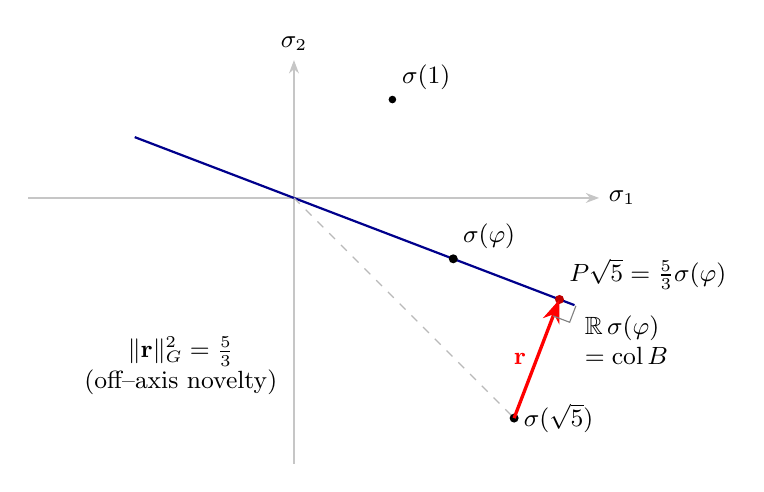
\begin{tikzpicture}[scale=1.25,>={Stealth[]},font=\small]
  \draw[gray!45,->] (-2.7,0) -- (3.1,0) node[right,black]{$\sigma_1$};
  \draw[gray!45,->] (0,-2.7) -- (0,1.4) node[above,black]{$\sigma_2$};
  \draw[thick,blue!55!black] (-1.618,0.618) -- (2.85,-1.089)
        node[below right,black,align=left]{$\R\,\sigma(\varphi)$\\$=\col\BB$};
  \coordinate (O) at (0,0);
  \coordinate (phi) at (1.618,-0.618);
  \coordinate (r5) at (2.236,-2.236);
  \coordinate (proj) at (2.697,-1.031);
  \draw[gray!55,dashed] (O) -- (r5);
  \fill (1,1) circle (1.1pt) node[above right]{$\sigma(1)$};
  \fill (phi) circle (1.3pt) node[above right]{$\sigma(\varphi)$};
  \fill (r5) circle (1.3pt) node[right]{$\sigma(\sqrt5)$};
  \fill[red!75!black] (proj) circle (1.3pt) node[above right,black]{$P\sqrt5=\tfrac53\sigma(\varphi)$};
  \draw[red,very thick,->] (r5) -- (proj) node[midway,left]{$\rr$};
  \draw[gray] (2.865,-1.095) -- (2.801,-1.263) -- (2.633,-1.199);
  \node[align=center] at (-1.15,-1.7) {$\lVert\rr\rVert_{\GG}^2=\tfrac53$\\(off--axis novelty)};
\end{tikzpicture}
\caption{The projector and residual of Examples~\ref{ex:proj5} and~\ref{ex:natgrad}, drawn in the Minkowski
plane of $\Q(\sqrt5)$ where the trace metric $\GG$ \emph{is} the Euclidean metric. The forced line is
$\col\BB=\R\,\sigma(\varphi)$; the point $\sigma(\sqrt5)$ projects $\GG$--orthogonally to
$P\sqrt5=\tfrac53\,\sigma(\varphi)$, and the perpendicular drop is the residual $\rr$ with
$\lVert\rr\rVert_{\GG}^2=\tfrac53$.}
\label{fig:proj}
\end{figure}

\begin{example}[A complex--embedding projector]\label{ex:complexproj}
We carry $\Q(i)$ through the projector with its Hermitian Gram $G_2=2I$ (\S\ref{subsec:complex}, positive
definite). With forced basis $\BB=\langle 1\rangle=(1,0)\transpose$ and target $x=i=(0,1)\transpose$, one has
$\BB^{*}G_2\BB=2$ and $\BB^{*}G_2 x=0$, so $Px=0$ and $\rr=i$ with
$\lVert\rr\rVert_{G_2}^2=(0,1)\,G_2\,(0,1)\transpose=2$. The residual is all of $i$: it is $G_2$--orthogonal to
$1$ (indeed $\Tr_{\Q(i)/\Q}(i)=0$), so $i$ is pure off--axis novelty against $\langle1\rangle$. The exact
projector/residual calculus thus runs verbatim over the Hermitian form when $r_2>0$; what remains open (O2) is
the probe--level verification of the Fisher identities in the genuinely complex case, which we flag rather
than assert.
\end{example}

\subsection{Understanding as zero residual}
Equation~\eqref{eq:capture} is the framework's operational definition of \emph{captured} (``understood''):
$\xx$ is explained by the current dictionary exactly when $\rr(\xx)=0$. A persistently nonzero residual is
the signal that the dictionary is too small---the object to be learned. The orthogonality
$\BB\transpose\GG\rr=0$ guarantees that the residual carries no component already in the forced subspace; it
is pure novelty.

\subsection{Trace duality: dual basis, codifferent, and different}\label{subsec:dual}
The inverse Gram $\GG\inv$ in the projector $P=\BB(\BB\transpose\GG\BB)\inv\BB\transpose\GG$ is not an
analytic convenience; it is the matrix of \emph{trace duality}. For a basis $\{\omega_i\}$ of $\K$ the dual
basis $\{\omega_i^\vee\}$ is defined by $\Tr(\omega_i\omega_j^\vee)=\delta_{ij}$, and in coordinates
$\omega_i^\vee=\sum_j(\GG\inv)_{ij}\omega_j$, since
$\Tr(\omega_i\,\omega_j^\vee)=\sum_k(\GG\inv)_{jk}\GG_{ki}=(\GG\inv\GG)_{ji}=\delta_{ij}$. The lattice
$L=\bigoplus_i\Z\omega_i$ has \emph{dual lattice}
\[
  L^\vee=\{x\in\K:\Tr(xL)\subseteq\Z\}=\bigoplus_i\Z\,\omega_i^\vee,
\]
and for $L=\OK$ this is the \emph{codifferent} $\OK^\vee\supseteq\OK$, a fractional ideal whose inverse is
the \emph{different} $\mathfrak d=(\OK^\vee)\inv\subseteq\OK$. Trace duality binds the metric to the
discriminant: for an integral basis $\det\GG=d_\K$, and the different computes the discriminant as a norm,
$\mathrm N(\mathfrak d)=|d_\K|$. For a non--maximal order $\Z[\theta]\subseteq\OK$ the trace--form
determinant carries the index,
\[
  \disc(\Z[\theta])=[\OK:\Z[\theta]]^2\,d_\K ,
\]
so $\det\GG$ in a power basis already measures how far $\theta$ is from generating the full ring of integers.

\begin{example}[Trace duality in $\Q(\sqrt5)$]\label{ex:dual}
With basis $\{1,\varphi\}$, $\GG=\left(\begin{smallmatrix}2&1\\1&3\end{smallmatrix}\right)$,
$\det\GG=5=d_{\Q(\sqrt5)}$ and $\GG\inv=\tfrac15\left(\begin{smallmatrix}3&-1\\-1&2\end{smallmatrix}\right)$.
The dual basis is $1^\vee=\tfrac15(3-\varphi)$ and $\varphi^\vee=\tfrac15(2\varphi-1)$; one checks
$\Tr(1\cdot 1^\vee)=\tfrac15\big(3\Tr 1-\Tr\varphi\big)=\tfrac15(6-1)=1$ and
$\Tr(\varphi\cdot 1^\vee)=\tfrac15\big(3\Tr\varphi-\Tr\varphi^2\big)=\tfrac15(3-3)=0$. The different is
$\mathfrak d=(m'(\varphi))=(2\varphi-1)=(\sqrt5)$ with $\mathrm N(\mathfrak d)=5=|d_\K|$, and
$\OK^\vee=\tfrac1{\sqrt5}\OK$.
\end{example}

\begin{remark}[Why this matters for learning]\label{rem:dual}
The residual $\rr=x-Px$ is the component of $x$ that pairs to zero, under $\Tr$, against the whole forced
subspace---the part of $x$ \emph{invisible to the current dictionary in the trace pairing}. Capturing it
(\S\ref{sec:learning}) adjoins the missing dual direction. Projector, residual, and dual lattice are thus
three views of one object: the trace form and its inverse.
\end{remark}

\begin{remark}[Galois invariance of capture]\label{rem:galois}
The trace pairing is invariant under every automorphism $g$ of $\K/\Q$: since $g$ permutes the embeddings
$\sigma_k$, we have $\Tr(g(x)g(y))=\Tr(g(xy))=\Tr(xy)$. Hence if $\K/\Q$ is Galois, $\mathrm{Gal}(\K/\Q)$ acts by
$\GG$--isometries ($g\transpose\GG g=\GG$ on coordinates); a Galois--stable forced subspace has a
Galois--stable residual, and ``captured'' ($\rr=0$) is a Galois--invariant notion. The learner's geometry
respects the arithmetic symmetry of the field.
\end{remark}

\section{Learning as exact basis growth}\label{sec:learning}

\subsection{The residual is the loss}
In place of a differentiable loss minimised by gradient descent, the framework uses the exact residual as
its error signal. The Pythagorean decomposition
\begin{equation}\label{eq:pythagoras}
  \lVert\xx\rVert_{\GG}^2=\lVert P\xx\rVert_{\GG}^2+\lVert\rr(\xx)\rVert_{\GG}^2
\end{equation}
(immediate from $\GG$--orthogonality of $P\xx$ and $\rr$) splits each observation into a captured part and a
residual; learning drives the residual to zero by enlarging $\col(\BB)$.

\subsection{The propose--for--confirm protocol and guardrails}\label{subsec:protocol}
Growth is disciplined. We summarise the invariants that the implementation maintains; they are not theorems
about $\K$ but design guarantees that keep the learner exact and auditable.

\begin{protocol}[Gated, witnessed growth]\label{prot:growth}
A streaming learner maintains a forced basis $\BB$, an exact residual--field accumulator (a running mean of
$\rr$ over consecutive off--axis observations), and a persistence counter. It exposes three operations:
\begin{enumerate}[label=(\alph*),leftmargin=*]
  \item \emph{observe}$(\xx)$: compute $\rr(\xx)$ and update the accumulator; never mutates $\BB$;
  \item \emph{propose}$()$: when the residual centroid has persisted and a capacity gate
        (\S\ref{sec:capacity}) admits the implied seed, return a candidate algebraic--integer seed; pure;
  \item \emph{confirm}$(\text{seed})$: the \emph{sole} mutator---adjoin the seed's coordinate vector to
        $\BB$, re--derive $P$, and append the growth to a SHA--256 witness chain.
\end{enumerate}
\end{protocol}

The maintained invariants are: \emph{(exactness)} every quantity entering a membership or admissibility
decision is a $\Q$/$\Z$ value, floats appearing only in display; \emph{(algebraic integrality)} every seed
is a monic--integer minimal polynomial; \emph{(sole mutator)} only \emph{confirm} changes $\BB$;
\emph{(witnessed)} each growth is a tamper--evident, replayable record. These are the guardrails that let one
trust the learner's output bit--for--bit.

\subsection{The coordinates--to--minimal--polynomial bridge}\label{subsec:bridge}
A residual centroid is a coordinate vector; to adjoin it as a named algebraic--integer seed we need its
minimal polynomial. We compute it exactly.

\begin{theorem}[Exact seed identity]\label{thm:bridge}
Let $\alpha=\sum_i a_i\theta^{i}\in\K$ with $a_i\in\Q$, and let
$M_\alpha=\rho(\alpha)=\sum_i a_i\,C(m_\theta)^{i}$ be its matrix under $\rho$. Then $m_\alpha$,
the minimal polynomial of $\alpha$ over $\Q$, equals the largest invariant factor of $xI-M_\alpha$, computed
by Smith normal form over $\Q[x]$. If $\alpha\in\OK$ (an algebraic integer) then $m_\alpha\in\Z[x]$ is monic;
otherwise the computation produces a non--integer monic polynomial and the seed is rejected.
\end{theorem}
\begin{proof}
$M_\alpha$ is exactly the matrix of multiplication by $\alpha$, so $\minpoly(M_\alpha)=m_\alpha$ by
Proposition~\ref{prop:regrep}, and this is the largest invariant factor by Corollary~\ref{cor:largestif}.
Integrality of $m_\alpha$ for $\alpha\in\OK$ is the defining property of algebraic integers; the converse
guards the seed dictionary against non--integral elements.
\end{proof}

\begin{example}[The bridge, worked]\label{ex:bridge}
In $\K=\Q(\theta)$, $\theta=\sqrt2+\sqrt3$, $m_\theta=x^4-10x^2+1$, the companion matrix and the
regular--representation of $2\sqrt6=\theta^2-5$ (coordinate vector $(-5,0,1,0)$) are
\[
  \rho(\theta)=\begin{pmatrix}0&0&0&-1\\1&0&0&0\\0&1&0&10\\0&0&1&0\end{pmatrix},\qquad
  \rho(2\sqrt6)=\rho(\theta)^2-5I=\begin{pmatrix}-5&0&-1&0\\0&-5&0&-1\\1&0&5&0\\0&1&0&5\end{pmatrix}.
\]
Reducing $xI-\rho(2\sqrt6)$ to Smith normal form over $\Q[x]$ gives $\diag(1,1,\,x^2-24,\,x^2-24)$, so the
invariant factors are $(x^2-24,\,x^2-24)$ and the largest---hence $m_{2\sqrt6}$---is $x^2-24$. This matches
the elementary check $(2\sqrt6)^2=24$, and the doubled factor reflects $n/d=4/2=2$
(Proposition~\ref{prop:regrep}). The polynomial is monic over $\Z$, so $2\sqrt6$ is admitted as an
algebraic--integer seed.
\end{example}

\subsection{Cross--field growth and the compositum}\label{subsec:compositum}
Some residuals are not elements of $\K$ at all: the observed algebraic quantity is forced into a strictly
larger field. Capturing it requires not a new vector but a new \emph{field}. We work in the
\emph{disjoint} (linearly disjoint) case.

\begin{definition}[Linear disjointness]\label{def:disjoint}
Finite extensions $\K,L/\Q$ are linearly disjoint if $\K\otimes_\Q L\to \K L$ is injective, equivalently
$[\K L:\Q]=[\K:\Q]\,[L:\Q]$, equivalently $\{e_if_j\}$ is a $\Q$--basis of $\K L$ for $\Q$--bases
$\{e_i\}$ of $\K$ and $\{f_j\}$ of $L$.
\end{definition}

\begin{proposition}[Kronecker Gram of a disjoint compositum]\label{prop:kron}
If $\K,L$ are linearly disjoint with bases $\{e_i\}$ ($i\le m$) and $\{f_j\}$ ($j\le k$), then the
trace--form Gram of $\K L$ on the product basis $\{e_if_j\}$ factors as
\begin{equation}\label{eq:kron}
  \GG_{\K L}=\GG_\K\otimes\GG_L,\qquad
  \det\GG_{\K L}=(\det\GG_\K)^{k}(\det\GG_L)^{m}.
\end{equation}
\end{proposition}
\begin{proof}
The embeddings of the disjoint compositum are exactly the products $\tau\otimes\upsilon$ of an embedding
$\tau$ of $\K$ and an embedding $\upsilon$ of $L$, and on $a\in\K,\,b\in L$ one has
$(\tau\otimes\upsilon)(ab)=\tau(a)\upsilon(b)$. Hence for $a\in\K,\,b\in L$,
\[
  \Tr_{\K L/\Q}(ab)=\sum_{\tau,\upsilon}\tau(a)\upsilon(b)
  =\Big(\sum_\tau\tau(a)\Big)\Big(\sum_\upsilon\upsilon(b)\Big)=\Tr_{\K/\Q}(a)\,\Tr_{L/\Q}(b).
\]
Applying this to $a=e_ie_{i'}$, $b=f_jf_{j'}$ gives
\begin{align*}
  (\GG_{\K L})_{(i,j),(i',j')}
  &=\Tr_\K(e_ie_{i'})\,\Tr_L(f_jf_{j'})\\
  &=(\GG_\K)_{ii'}(\GG_L)_{jj'},
\end{align*}
which is the Kronecker product. The determinant in~\eqref{eq:kron} is the standard identity
\[
  \det(A\otimes B)=(\det A)^{\dim B}(\det B)^{\dim A},\qquad \dim\GG_\K=m,\ \dim\GG_L=k.
\]
\end{proof}

\begin{corollary}[Multiquadratic tower]\label{cor:tower}
For pairwise linearly disjoint $\K_1,\dots,\K_r$, iterating~\eqref{eq:kron} gives
$\GG_{\K_1\cdots\K_r}=\GG_{\K_1}\otimes\cdots\otimes\GG_{\K_r}$. In particular
$\Q(\sqrt{p_1},\dots,\sqrt{p_r})$ for distinct primes $p_i$ has, on the $2^r$ squarefree--product basis,
$\GG=\bigotimes_{i=1}^r\left(\begin{smallmatrix}2&0\\0&2p_i\end{smallmatrix}\right)$---a diagonal matrix of
order $2^r$ with entries $2^r\prod_{i\in S}p_i$ over subsets $S\subseteq\{1,\dots,r\}$. For $\{p_i\}=\{2,3\}$
this is $\diag(4,8,12,24)$, recovering Example~\ref{ex:biquad}.
\end{corollary}

\begin{example}[Adjoining $\sqrt7$]\label{ex:adjoin7}
$\K=\Q(\sqrt2,\sqrt3)$ ($\GG_\K=\diag(4,8,12,24)$) and $L=\Q(\sqrt7)$ ($\GG_L=\diag(2,14)$) are linearly
disjoint, since $[\K L:\Q]=8=4\cdot 2$. By~\eqref{eq:kron},
\[
  \GG_{\K L}=\GG_\K\otimes\GG_L=\diag(8,56,16,112,24,168,48,336),\qquad
  \det\GG_{\K L}=9216^2\cdot 28^4 .
\]
After adjoining $\sqrt7$ the previously out--of--field residual is captured and its field residual returns
to $0$.
\end{example}

\begin{remark}[The non--disjoint case is open]\label{rem:nondisjoint}
When the candidate generator's minimal polynomial \emph{partially factors} over $\K$, the compositum is
strictly smaller than the tensor product, $[\K(\beta):\K]<\deg m_\beta$, and~\eqref{eq:kron} no longer
applies; one must build the true compositum basis (e.g. via a primitive element and resultants, with
factorisation over a number field). This is a genuine open extension of the present work; the implemented
learner detects it and refuses growth rather than producing a fictitious Gram.
\end{remark}

\begin{example}[A non--disjoint extension]\label{ex:nondisjoint}
Over $\K=\Q(\sqrt2)$ adjoin $\beta=\sqrt2+\sqrt3$, whose minimal polynomial over $\Q$ is $x^4-10x^2+1$. Over
$\K$ this polynomial \emph{factors}:
\[
  x^4-10x^2+1=(x^2+2\sqrt2\,x-1)(x^2-2\sqrt2\,x-1)\quad\text{in }\Q(\sqrt2)[x],
\]
since $2\sqrt2\in\K$ (one checks $\beta^2-2\sqrt2\,\beta-1=0$). Hence $[\K(\beta):\K]=2<4=\deg m_\beta$, so
$\K$ and $\Q(\beta)$ are \emph{not} linearly disjoint. The true compositum $\K(\beta)=\Q(\sqrt2,\sqrt3)$ has
degree $4$, not the tensor degree $[\K:\Q]\deg m_\beta=2\cdot4=8$; the Kronecker Gram
$\GG_\K\otimes\GG_{\Q(\beta)}$ would describe an $8$--dimensional space that does not exist. The learner
detects the partial factorisation and refuses growth (Remark~\ref{rem:nondisjoint}); constructing the correct
degree--$4$ Gram requires a primitive element of $\K(\beta)$ and is left open.
\end{example}

\section{Capacity control via heights}\label{sec:capacity}

Unbounded basis growth would defeat the purpose of an exact, finite model. We bound capacity by arithmetic
height, which makes the admissible seed set provably finite.

\subsection{Mahler measure and height}
\begin{definition}[Mahler measure]\label{def:mahler}
For $p(x)=a_n\prod_{i}(x-\alpha_i)\in\C[x]$, $\Mah(p)=|a_n|\prod_i\max(1,|\alpha_i|)$. For an algebraic
$\theta$ with minimal polynomial $m_\theta$ over $\Z$ (primitive integer form), $\Mah(\theta)=\Mah(m_\theta)$.
\end{definition}

\begin{theorem}[Height, Landau, Northcott]\label{thm:height}
Let $p\in\Z[x]$ be monic of degree $d$ with coefficient vector $(1,c_{d-1},\dots,c_0)$.
\begin{enumerate}[label=(\alph*),leftmargin=*]
  \item $\Mah(\theta)=\height(\theta)^{\deg\theta}$, where $\height$ is the absolute multiplicative Weil
        height \cite{BombieriGubler}.
  \item \emph{(Landau)} $\Mah(p)\le \lVert p\rVert_2=\big(\sum_i c_i^2\big)^{1/2}$, hence
        $\Mah(p)^2\le \sum_i c_i^2\in\Z$.
  \item \emph{(Northcott)} For each $D,B$ there are only finitely many algebraic integers $\theta$ with
        $\deg\theta\le D$ and $\Mah(\theta)\le B$ \cite{Northcott}.
\end{enumerate}
\end{theorem}
\begin{proof}
(a) is the definition of the Weil height via local contributions \cite{BombieriGubler}. (b) is Landau's
inequality \cite{Landau,Mahler}. (c): a monic integer polynomial of degree $\le D$ with $\Mah\le B$ has, by
Mahler's coefficient bound $|c_j|\le\binom{d}{j}\Mah(p)$, bounded integer coefficients, so there are finitely
many such polynomials, hence finitely many such $\theta$.
\end{proof}

\begin{figure}[ht]
\centering
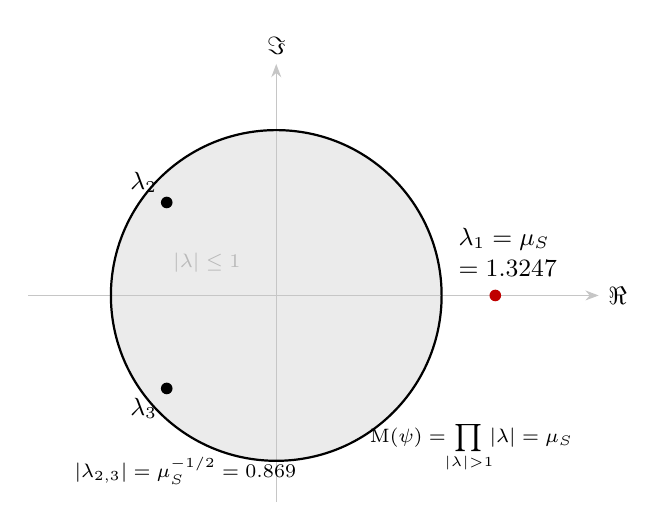
\begin{tikzpicture}[scale=2.1,>={Stealth[]},font=\small]
  \fill[black!8] (0,0) circle (1);
  \draw[gray!45,->] (-1.5,0) -- (1.95,0) node[right,black]{$\Re$};
  \draw[gray!45,->] (0,-1.25) -- (0,1.4) node[above,black]{$\Im$};
  \draw[thick] (0,0) circle (1);
  \node[gray!55] at (-0.42,0.2) {\scriptsize $|\lambda|\le1$};
  \fill[red!75!black] (1.3247,0) circle (1.0pt);
  \node[black,align=left] at (1.40,0.26) {$\lambda_1=\mu_S$\\$=1.3247$};
  \fill (-0.6624,0.5623) circle (1.0pt) node[above left]{$\lambda_2$};
  \fill (-0.6624,-0.5623) circle (1.0pt) node[below left]{$\lambda_3$};
  \node[align=left] at (-0.55,-1.06) {\scriptsize $|\lambda_{2,3}|=\mu_S^{-1/2}=0.869$};
  \node[align=center] at (1.18,-0.92) {\scriptsize $\Mah(\psi)=\!\!\displaystyle\prod_{|\lambda|>1}\!\!|\lambda|=\mu_S$};
\end{tikzpicture}
\caption{The Mahler picture for the plastic number $\psi$ (Smyth's minimiser, root of $x^3-x-1$): the
eigenvalues of $\rho(\psi)=C(x^3-x-1)$ plotted in $\C$ with the unit circle. Only $\lambda_1=\psi$ lies
outside, so $\Mah(\psi)=\prod_{|\lambda|>1}|\lambda|=\mu_S=1.3247\ldots$ (Remark~\ref{rem:mahlerspectral}).
Smyth's bound $\mu_S$ is a theorem for non--reciprocal integers (Theorem~\ref{thm:smythfloor}); Lehmer's
conjectural universal floor is the smaller $\mu_L=1.17628\ldots$.}
\label{fig:mahler}
\end{figure}

\subsection{The exact admissibility gate}
Define the \emph{degree} $\deg(m)$ and the integer \emph{coefficient height}
$\operatorname{ch}(m)=\max_i|c_i|$. A \emph{budget} is a pair $(D_{\max},H_{\max})\in\Z^2$.

\begin{definition}[Northcott admissibility]\label{def:admissible}
$m$ is \emph{admissible} for $(D_{\max},H_{\max})$ iff $\deg(m)\le D_{\max}$ and
$\operatorname{ch}(m)\le H_{\max}$.
\end{definition}

\begin{proposition}[Bounded capacity, exact gate]\label{prop:cap}
The admissible set $\{\,m\in\Z[x]\text{ monic}: \deg m\le D_{\max},\ \operatorname{ch}(m)\le H_{\max}\,\}$ is
finite, of size $\sum_{d=1}^{D_{\max}}(2H_{\max}+1)^{d}$. The predicate of
Definition~\ref{def:admissible} is decided entirely in $\Z$; the Mahler measure $\Mah(m)$ never enters it,
and the exact integer $\sum_i c_i^2$ certifies $\Mah(m)^2\le\sum_i c_i^2$ by Theorem~\ref{thm:height}(b).
\end{proposition}
\begin{proof}
Each of the $d$ non--leading coefficients ranges over the $2H_{\max}+1$ integers in
$[-H_{\max},H_{\max}]$, and the leading coefficient is $1$; summing over $1\le d\le D_{\max}$ gives the count.
Finiteness is the constructive form of Northcott (Theorem~\ref{thm:height}(c)). The decision uses only the
integer comparisons $\deg\le D_{\max}$ and $\operatorname{ch}\le H_{\max}$.
\end{proof}

\begin{example}[Northcott finiteness, concretely]\label{ex:northcott}
Under the budget $D_{\max}=2,\ H_{\max}=1$ the admissible monic integer polynomials number
$\sum_{d=1}^{2}3^{d}=3+9=12$: the three linear $x+c$ ($c\in\{-1,0,1\}$) and the nine quadratics $x^2+bx+c$
($b,c\in\{-1,0,1\}$). Finiteness is not asymptotic---the entire admissible set is small and listable. Among
the quadratics, $x^2-x-1$ (the golden seed $\varphi$) and $x^2+x-1$ are irreducible; $x^2-1$ and $x^2+x$ are
reducible and define no new field; $x^2+1$ cuts out $\Q(i)$ (Example~\ref{ex:gaussint}). Raising $H_{\max}$
to $24$ first admits $2\sqrt6$ ($x^2-24$); the budget is precisely the dial that bounds an explicitly
enumerable dictionary.
\end{example}

\begin{example}[Exact heights]\label{ex:heights}
The following are computed exactly (no roots, no floats):
\begin{center}
\begin{tabular}{lcccc}
\toprule
seed & minimal polynomial & $\deg$ & $\operatorname{ch}$ & $\sum c_i^2$ \\
\midrule
$\varphi$ & $x^2-x-1$ & $2$ & $1$ & $3$ \\
$2\sqrt6$ & $x^2-24$ & $2$ & $24$ & $577$ \\
$\sqrt7$ & $x^2-7$ & $2$ & $7$ & $50$ \\
$\mathrm{gap}=\varphi^4$ & $x^2-7x+1$ & $2$ & $7$ & $51$ \\
\bottomrule
\end{tabular}
\end{center}
Landau is tight here: $\Mah(2\sqrt6)=24$ and $24^2=576\le 577=\sum c_i^2$.
\end{example}

\begin{remark}[The float never crosses the gate]\label{rem:floatgate}
The Mahler measure is a float (it requires the complex roots). For instance the exact value $\Mah(\sqrt7)=7$
is computed by a root finder as $7.000000000000001$---strictly above $7$. A naive floating test
``$\Mah\le 7$'' would erroneously reject $\sqrt7$ on rounding noise; the integer gate of
Definition~\ref{def:admissible} cannot. The admissibility decision depends only on
$(\deg,\operatorname{ch})$ and is invariant to the float Mahler value.
\end{remark}

The growth gate $\textsc{capacity\_decision}$ returns one of $\textsc{grow}/\textsc{stop}/\textsc{reject}$:
\textsc{reject} if the seed is inadmissible (Definition~\ref{def:admissible}); \textsc{stop} if the residual
defect is below a floor; and \textsc{grow} otherwise. The floor is the subject of \S\ref{sec:threshold}; in
the shipped gate it is $0$ (any nonzero defect passes), a choice we revisit there.

\section{A worked learning episode}\label{sec:episode}
We trace the full loop in $\K=\Q(\sqrt2+\sqrt3)=\Q[x]/(x^4-10x^2+1)$ (degree $n=4$, so
$\K=\Q(\sqrt2,\sqrt3)$), with forced basis $\BB=\{1,\theta\}$, $\theta=\sqrt2+\sqrt3$, so
$\col(\BB)=\Q\oplus\Q\theta$.

\paragraph{In--distribution.} Any observation $a+b\theta$ ($a,b\in\Q$) lies in $\col(\BB)$, so $\rr=0$:
captured, nothing proposed.

\paragraph{Persistent off--axis novelty.} Stream observations $\xx=u+2\sqrt6$ with $u\in\col(\BB)$, where
$2\sqrt6=\theta^2-5$ has coordinate vector $(-5,0,1,0)$ and is $\GG$--orthogonal to $\col(\BB)$. Then
$\rr(\xx)=2\sqrt6$ exactly, and, the trace being basis--independent,
\[
  \lVert\rr\rVert_{\GG}^2=T(2\sqrt6,2\sqrt6)=\Tr_{\K/\Q}\!\big((2\sqrt6)^2\big)=\Tr_{\K/\Q}(24)=4\cdot24=96 .
\]
As an exact check, for $\xx=\theta+2\sqrt6$ the Pythagorean split~\eqref{eq:pythagoras} reads
$\lVert\xx\rVert_{\GG}^2=116=20+96$, with captured part $\lVert\theta\rVert_{\GG}^2=\Tr(\theta^2)=20$,
residual $\lVert\rr\rVert_{\GG}^2=96$, and vanishing cross term $\Tr(\theta\cdot 2\sqrt6)=0$.
Once the persistence count is met, \emph{propose} returns the exact seed identity (Theorem~\ref{thm:bridge})
$m_{2\sqrt6}=x^2-24$, of degree $2$ and coefficient height $24$ (Example~\ref{ex:heights}).

\paragraph{Capacity and threshold.} Under a budget $(D_{\max},H_{\max})=(64,256)$ the seed is admissible
($2\le 64$, $24\le 256$; Definition~\ref{def:admissible}). With the information rule~\eqref{eq:threshold} and
$\lambda=2$, the gain $96$ exceeds the cost $2\log24=6.36$ and the floor $0.562$, so the decision is
\textsc{grow}.

\paragraph{Confirm.} Adjoining $2\sqrt6$ to $\BB$ and re--deriving $P$---the sole mutation
(Protocol~\ref{prot:growth})---returns the residual of $u+2\sqrt6$ to $0$; the growth is appended to the
witness chain.

\paragraph{Out--of--field novelty.} Once the basis spans all of $\K$, so the captured field is
$\K=\Q(\sqrt2,\sqrt3)$ itself with $\GG_\K=\diag(4,8,12,24)$, suppose a quantity forced into
$\Q(\sqrt2,\sqrt3,\sqrt7)$ with a $\sqrt7$ component appears. Its field residual against $\K$ is nonzero, and
the candidate generator $\sqrt7$ ($m=x^2-7$) is linearly disjoint from $\K$ (Example~\ref{ex:adjoin7}).
Confirming the extension grows the field to the compositum with $\GG_{\K L}=\GG_\K\otimes\GG_L
=\diag(8,56,16,112,24,168,48,336)$ (Proposition~\ref{prop:kron}); the $\sqrt7$ residual then returns to $0$,
and the same height gate governs the decision on the actual compositum degree $4\to8$.

\section{Information geometry of the trace form}\label{sec:infogeo}

We read $\GG$, and the residual norm, as Fisher information. The two structural facts are \emph{classical}:
$\GG=M\transpose M$ (the trace form is the Minkowski--embedding Gram, Theorem~\ref{thm:GMM}; textbook
algebraic number theory \cite{Neukirch,Marcus}), and the Fisher information of a Gaussian location family
$\mathcal N(Ma,I)$ is $M\transpose M$ (the standard location--family formula \cite{Amari}). Our part is to
assemble these into a Fisher reading of the trace form, to pin the model--dependent conformal constant, and
to draw the residual--norm--as--information--distance consequence for the learner---not to resolve an open
mathematical problem. All displayed quantities are verified by exact symbolic computation
(Appendix~\ref{sec:appendix}); the choice of statistical model is not unique, and we are explicit about which
constant each model produces.

\subsection{Model 1: a Gaussian location family}
Let the field coordinate $a\in\R^d$ parameterise the \emph{mean} $\mu(a)=Ma$ of an isotropic Gaussian on the
Minkowski space, $\xx\sim\mathcal N(Ma,I_n)$, where $M$ is the embedding matrix~\eqref{eq:GandM}.

\begin{theorem}[Trace form is Gaussian Fisher information]\label{thm:gaussfisher}
For a totally real field, the Fisher information of the location family $\{\mathcal N(Ma,I_n)\}$ in the
parameter $a$ is
\[
  \Fish_{\mathrm{Gauss}}=M\transpose M=\GG .
\]
With covariance $cI_n$ in place of $I_n$, $\Fish_{\mathrm{Gauss}}=c\inv\GG$ (conformal, constant $c$).
\end{theorem}
\begin{proof}
For a Gaussian location family $\mathcal N(\mu(a),\Sigma)$, the Fisher information is
$(\partial\mu/\partial a)\transpose\Sigma\inv(\partial\mu/\partial a)$. Here $\partial\mu/\partial a=M$ and
$\Sigma=I_n$, so $\Fish=M\transpose M=\GG$ by Theorem~\ref{thm:GMM}; replacing $\Sigma$ by $cI_n$ scales by
$c\inv$.
\end{proof}

\begin{proposition}[The discriminant is an information volume]\label{prop:discvol}
Under Model~1 the Fisher information is the constant metric $\GG$ (Theorem~\ref{thm:gaussfisher}), so its
\emph{Jeffreys volume element}---the reparameterisation--invariant prior density $\sqrt{\det\Fish}$
\cite{Jeffreys}---is the constant $\sqrt{\det\GG}$. The Jeffreys volume of one fundamental cell of the
coordinate lattice (i.e. of $\OK$ in an integral basis) is therefore
\begin{equation}\label{eq:discvol}
  \operatorname{vol}_{\mathrm{Jeffreys}}=\int_{[0,1)^n}\!\sqrt{\det\GG}\,\,da=\sqrt{\det\GG}=\sqrt{|d_\K|},
\end{equation}
equal to the Minkowski covolume of $\sigma(\OK)$ (\S\ref{subsec:lattice}); for a sub--order of index $f$ it
scales by $f$. The square root of the field discriminant is the natural Fisher--Jeffreys volume of one lattice
cell of the statistical manifold.
\end{proposition}
\begin{proof}
For the location family $\mathcal N(Ma,I_n)$ the Fisher information is the constant $M\transpose M=\GG$
(Theorem~\ref{thm:gaussfisher}), independent of $a$; the Jeffreys density is then
$\sqrt{\det\Fish}=\sqrt{\det\GG}$ \cite{Jeffreys}, and integrating this constant over a unit coordinate cell
gives $\sqrt{\det\GG}$. By Theorem~\ref{thm:GMM}, $\det\GG=d_\K$ for an integral basis (and $f^2 d_\K$ for a
sub--order of index $f$), and $\sqrt{\det\GG}$ is the covolume.
\end{proof}

\begin{remark}[Discriminant as ``amount of arithmetic'']\label{rem:discvol}
The discriminant measures the arithmetic complexity of $\K$---its ramification. Equation~\eqref{eq:discvol}
reads it as an information volume: the larger $|d_\K|$, the more Fisher--Jeffreys volume one integer cell
occupies, so a more ramified field is, in a precise statistical sense, ``larger'' to learn. The covolumes
$\sqrt{|d_\K|}$ tabulated in Table~\ref{tab:catalog} ($\sqrt5,\,2\sqrt2,\,6\sqrt3$ for
$\Q(\sqrt5),\Q(\sqrt2),\Q(\sqrt[3]2)$) are exactly these information volumes.
\end{remark}

\begin{example}[Information volumes]\label{ex:jeffreys}
By Proposition~\ref{prop:discvol} the Jeffreys volume of one integer cell is $\sqrt{|d_\K|}$. From
Table~\ref{tab:catalog}: $\Q(\sqrt5)$ has volume $\sqrt5\approx2.236$, $\Q(\sqrt2)$ has
$2\sqrt2\approx2.828$, and the more ramified $\Q(\sqrt[3]2)$ has $6\sqrt3\approx10.39$---a single
$\OK$--cell of $\Q(\sqrt[3]2)$ thus occupies about $4.6$ times the Fisher--Jeffreys volume of a cell of
$\Q(\sqrt5)$. ``More ramified'' is here literally ``more information volume per lattice cell.''
\end{example}

\begin{remark}[The field's own description length]\label{rem:fieldmdl}
Proposition~\ref{prop:discvol} prices the \emph{field}, not just a seed. In an MDL/BIC account
\cite{Rissanen,Schwarz} a model's code length carries a term $\tfrac12\log\det(\text{Fisher})$; here that is
$\tfrac12\log\det\GG=\tfrac12\log|d_\K|=\log\sqrt{|d_\K|}=\log\operatorname{covol}(\Lambda_\K)$. The
description length of working in $\K$ is thus the logarithm of its Minkowski covolume---an Occam penalty on
ramification, complementing the per--seed entropy $\log\Mah$ of \S\ref{sec:threshold}.
\end{remark}

\begin{remark}[Information volume is the Model--1 reading]\label{rem:volmodel}
The volume $\sqrt{|d_\K|}$ of Proposition~\ref{prop:discvol} is the \emph{Model--1} ($c=1$) reading. Under the
maximum--entropy Model~2 the metric on the residual subspace is $\Fish_{\mathrm{exp}}=\GG/n$
(Theorem~\ref{thm:resfisher}), whose volume element rescales one cell by
$\det(\GG/n)^{1/2}=n^{-d/2}\sqrt{\det\GG}$. So ``information volume $=\sqrt{|d_\K|}$'' is model--dependent in
exactly the way Conjecture~\ref{conj:model} describes: the discriminant reading belongs to the Gaussian
model, the $n^{-d/2}$--scaled reading to the conjugate model. Model~1's manifold is moreover \emph{flat}
(constant Fisher $\GG$), so its content is the metric itself; any curvature of the statistical manifold lives
in Model~2.
\end{remark}

\subsection{Model 2: the maximum--entropy family on the conjugates}
The framework's canonical, zero--parameter measure is \emph{uniform} on the $n$ Galois conjugates. (For seeds
of growing degree this uniform--on--conjugates measure is the natural object of Bilu's equidistribution
theorem \cite{Bilu}, under which the conjugates equidistribute on the unit circle and the Mahler measure is an
integral over the limiting measure; it is natural here but not the only possible choice.) Consider
the discrete exponential family $p(k;a)\propto\exp\big((Ma)_k\big)$ on outcomes $k\in\{1,\dots,n\}$, with
sufficient statistic the embedding rows $s(k)=(\sigma_k(\omega_1),\dots,\sigma_k(\omega_d))$, and let
$t=(\Tr(\omega_1),\dots,\Tr(\omega_d))\transpose$ be the trace vector.

\begin{theorem}[Conjugate--family Fisher information]\label{thm:expfisher}
At the uniform point $a=0$ (so $p\equiv 1/n$), the Fisher information of $\{p(\cdot;a)\}$ is
\begin{equation}\label{eq:expfisher}
  \Fish_{\mathrm{exp}}=\frac1n\,\GG-\frac1{n^2}\,t\,t\transpose=\frac1n\Big(\GG-\frac1n\,t\,t\transpose\Big).
\end{equation}
\end{theorem}
\begin{proof}
For an exponential family the Fisher information equals the covariance of the sufficient statistic. At
$a=0$, $p$ is uniform, so
$\Cov[s_i,s_j]=\tfrac1n\sum_k\sigma_k(\omega_i)\sigma_k(\omega_j)-\big(\tfrac1n\sum_k\sigma_k(\omega_i)\big)
\big(\tfrac1n\sum_k\sigma_k(\omega_j)\big)=\tfrac1n\GG_{ij}-\tfrac1{n^2}t_it_j$, using
$\sum_k\sigma_k(\omega_i)\sigma_k(\omega_j)=\GG_{ij}$ (Theorem~\ref{thm:GMM}) and
$\sum_k\sigma_k(\omega_i)=\Tr(\omega_i)=t_i$.
\end{proof}

The correction $\tfrac1{n^2}tt\transpose$ is rank one, along the trace vector $t$. We isolate where it
vanishes.

\begin{lemma}[Trace--zero is the residual subspace]\label{lem:tracezero}
For a coordinate vector $v$, $\langle v,1\rangle_{\GG}=t\transpose v=\Tr(v)$, where $1=\omega_1$ is the
constant and $\Tr(v)$ denotes the trace of the field element with coordinates $v$. Consequently
$v\perp_{\GG}1\iff \Tr(v)=0\iff t\transpose v=0$. If the forced basis contains the constant
($1\in\col(\BB)$), then every residual $\rr=\xx-P\xx$ satisfies $\Tr(\rr)=0$.
\end{lemma}
\begin{proof}
$\langle v,1\rangle_{\GG}=v\transpose\GG e_1$. Since $\omega_1=1$, the first column of $\GG$ is
$(\Tr(\omega_i\cdot 1))_i=(\Tr(\omega_i))_i=t$, so $\langle v,1\rangle_{\GG}=t\transpose v
=\sum_i v_i\Tr(\omega_i)=\Tr(\sum_i v_i\omega_i)=\Tr(v)$. If $1\in\col(\BB)$ then
$\rr\perp_{\GG}\col(\BB)\ni 1$ (Proposition~\ref{prop:proj}), so $\Tr(\rr)=0$.
\end{proof}

\begin{theorem}[The residual norm is degree--scaled Fisher information]\label{thm:resfisher}
On the trace--zero subspace $\{v:t\transpose v=0\}$, $\GG=n\,\Fish_{\mathrm{exp}}$. In particular, if
$1\in\col(\BB)$ then for every residual $\rr$,
\begin{equation}\label{eq:resfisher}
  \lVert\rr\rVert_{\GG}^2=n\cdot\Fish_{\mathrm{exp}}(\rr) .
\end{equation}
\end{theorem}
\begin{proof}
For $t\transpose v=0$, \eqref{eq:expfisher} gives
$v\transpose\Fish_{\mathrm{exp}}v=\tfrac1n v\transpose\GG v-\tfrac1{n^2}(t\transpose v)^2=\tfrac1n
v\transpose\GG v$, i.e. $v\transpose\GG v=n\,v\transpose\Fish_{\mathrm{exp}}v$. By Lemma~\ref{lem:tracezero},
when $1\in\col(\BB)$ the residual $\rr$ is trace--zero, and~\eqref{eq:resfisher} is this identity at
$v=\rr$.
\end{proof}

\subsection{Exact evidence}
The matrices below are produced symbolically and verified exactly.
\begin{center}
\begin{tabular}{lccc}
\toprule
field (basis) & $n$ & $\GG$ & $\Fish_{\mathrm{exp}}$ \\
\midrule
$\Q(\sqrt5)$, $\{1,\varphi\}$ & $2$ & $\left(\begin{smallmatrix}2&1\\1&3\end{smallmatrix}\right)$ &
   $\left(\begin{smallmatrix}0&0\\0&5/4\end{smallmatrix}\right)$ \\[2pt]
$\Q(\sqrt2,\sqrt3)$, $\{1,\sqrt2,\sqrt3,\sqrt6\}$ & $4$ & $\diag(4,8,12,24)$ & $\diag(0,2,3,6)$ \\[2pt]
$\Q(\sqrt2,\sqrt3,\sqrt7)$ & $8$ & $\diag(8,56,16,112,24,168,48,336)$ & $\diag(0,7,2,14,3,21,6,42)$ \\
\bottomrule
\end{tabular}
\end{center}
In each case $\GG=M\transpose M$, $\Fish_{\mathrm{exp}}=\tfrac1n\GG-\tfrac1{n^2}tt\transpose$, and
$\GG=n\,\Fish_{\mathrm{exp}}$ on the trace--zero subspace. For a concrete residual, $\sqrt5=2\varphi-1$ has
coordinates $(-1,2)$, $\Tr(\sqrt5)=0$, and
\[
  \lVert\sqrt5\rVert_{\GG}^2=10=2\cdot 5=n\cdot\Fish_{\mathrm{exp}}(\sqrt5),
\]
matching~\eqref{eq:resfisher} with $n=2$.

\subsection{Relative entropy and natural gradient}
Both identifications are local forms of relative entropy. For a smooth family $\{p_a\}$ the
Kullback--Leibler divergence expands to second order as
\[
  D_{\mathrm{KL}}\!\big(p_{a}\,\Vert\,p_{a+\delta}\big)=\tfrac12\,\delta\transpose\Fish(a)\,\delta
  +O(\lVert\delta\rVert^3),
\]
so the Fisher matrix is the Riemannian metric of the statistical manifold \cite{AmariNagaoka}. By
Theorems~\ref{thm:gaussfisher} and~\ref{thm:resfisher}, $\GG$ (respectively $n\inv\GG$ on the residual
subspace) \emph{is} that metric. Consequently a step measured in $\lVert\cdot\rVert_{\GG}$ is a
natural--gradient step \cite{Amari}, and $\lVert\rr\rVert_{\GG}^2$ is twice the leading Kullback--Leibler
cost of failing to capture $\rr$. This is the precise sense in which the residual norm is an information
distance rather than a merely Euclidean one; it is the analytic content used in \S\ref{sec:threshold}.

\begin{proposition}[The projector is a one--step natural--gradient fit]\label{prop:natgrad}
Fix $x\in\K$ and the forced basis $\BB$, and consider the quadratic loss
$L(a)=\tfrac12\lVert x-\BB a\rVert_{\GG}^2$ on coordinate vectors $a$. In the $\GG$--geometry its gradient and
Hessian are $\nabla L(a)=\BB\transpose\GG(\BB a-x)$ and $\nabla^2 L=\BB\transpose\GG\BB$, so the
natural--gradient (Newton) step from $a=0$ lands at $a^\star=(\BB\transpose\GG\BB)\inv\BB\transpose\GG x$.
Then $\BB a^\star=Px$ and the optimal residual is $x-Px=\rr$: the trace--form natural gradient solves the
exact--fit problem in a single step, and its fixed point is the projector of Proposition~\ref{prop:proj}.
\end{proposition}
\begin{proof}
The gradient and Hessian are immediate, and $L$ is quadratic, so the single Newton step
$a^\star=-(\nabla^2L)\inv\nabla L(0)=(\BB\transpose\GG\BB)\inv\BB\transpose\GG x$ is exact; then
$\BB a^\star=\BB(\BB\transpose\GG\BB)\inv\BB\transpose\GG x=Px$ by the definition of $P$, and the residual is
$x-Px=\rr$.
\end{proof}
\begin{remark}
Because the loss is quadratic with Hessian $\GG$, the natural gradient \emph{is} the Newton step: learning the
captured part of $x$ takes one exact step, not an iterative descent. This is the optimisation shadow of the
idempotence $P^2=P$ (Proposition~\ref{prop:proj})---re--fitting an already--captured $x$ moves nothing.
\end{remark}

\begin{example}[One--step fit in $\Q(\sqrt5)$]\label{ex:natgrad}
Take $\BB=\langle\varphi\rangle$ (so $\BB=(0,1)\transpose$), $\GG=\left(\begin{smallmatrix}2&1\\1&3\end{smallmatrix}\right)$,
and target $x=\sqrt5=(-1,2)\transpose$ (Example~\ref{ex:proj5}). The natural--gradient step is
$a^\star=(\BB\transpose\GG\BB)\inv\BB\transpose\GG x=3\inv\!\cdot 5=\tfrac53$, giving
$Px=(0,\tfrac53)\transpose$ and residual $\rr=(-1,\tfrac13)\transpose$ with
$\lVert\rr\rVert_{\GG}^2=\tfrac53$ in a single move---exactly the projector of Example~\ref{ex:proj5}, now
realised as a one--step Newton fit. A Euclidean step would use $\BB\transpose\BB=1$ in place of
$\BB\transpose\GG\BB=3$ and land off the $\GG$--projection.
\end{example}

\subsection{Honest caveats}
\begin{conjecture}[No canonical model]\label{conj:model}
There is no model--independent identification of $\GG$ with ``the'' Fisher metric of the substrate. Two
natural models give two constants: $\GG=\Fish_{\mathrm{Gauss}}$ ($c=1$, whole space,
Theorem~\ref{thm:gaussfisher}) and $\GG=n\,\Fish_{\mathrm{exp}}$ ($c=n$, residual subspace,
Theorem~\ref{thm:resfisher}). Which model is canonical is an interpretive choice, not forced by the field.
By \v{C}encov's theorem the Fisher metric is the unique Riemannian metric invariant under sufficient
statistics \emph{up to scale} \cite{Cencov}; the $c=1$ versus $c=n$ ambiguity is therefore a choice of model
\emph{and} of that scale, not a choice of a different metric. The companion paper names a third,
framework--native scale---the self--action eigenframe gap $c=\sqrt{1+4C}/(2C)$ at a critical point of the
ladder $x^2+x=C$ (golden gate $c=\sqrt5/2$)---under which the exchange rate is the identity $\lambda=2c$; by the
present conjecture this is a principled \emph{selection} of $c$, not a removal of the freedom it identifies.
\end{conjecture}
\begin{remark}[Two further caveats]\label{rem:fishercaveats}
\emph{(i) Complex embeddings.} Theorems~\ref{thm:GMM}--\ref{thm:resfisher} are stated for totally real fields.
For $r_2>0$ the trace form is indefinite; the positive--definite Hermitian form $G_2=M^{*}M$ of
\S\ref{subsec:complex} replaces $\GG$, and the identities carry over with $G_2$ in its place---the isotropic
Gaussian of Theorem~\ref{thm:gaussfisher} taken on the canonical real Minkowski space $\R^n$, whose
embedding Jacobian $J$ satisfies $J\transpose J=G_2$. The worked examples in this section are totally real and
use $\GG$ directly; an exact probe on a field with $r_2>0$ is left to future work (O2).
\emph{(ii) The $1\in\col(\BB)$ condition.} Identity~\eqref{eq:resfisher} requires the constant to lie in the
forced basis (Lemma~\ref{lem:tracezero}). The constant is \emph{not} auto--injected; ``$\rr\perp_{\GG}1$''
is therefore a usage convention, true only when $1\in\col(\BB)$. When $1\notin\col(\BB)$ the residual can
carry a nonzero--trace component and~\eqref{eq:resfisher} fails. This is verified both ways in the probe: in
$\Q(\sqrt5)$, projecting onto $\langle 1\rangle$ gives a trace--zero residual, while projecting onto
$\langle\varphi\rangle$ leaves the residual of $1$ with trace $5/3\neq 0$.
\end{remark}

\section{The growth threshold}\label{sec:threshold}

We now ask the operational question (the ``residual--enlargement'' rule, denoted R1 in the project): how
large must $\lVert\rr\rVert_{\GG}$ be to justify adjoining a seed of arithmetic height? We frame it as
information gained versus information spent, using Theorem~\ref{thm:resfisher}.

\subsection{Gain versus cost}
\begin{definition}[Information gain and cost]\label{def:gaincost}
For a residual $\rr$ (with $1\in\col(\BB)$) and a candidate seed $\theta$ of degree $d$ and Mahler measure
$\Mah(\theta)=\height(\theta)^d$, set
\[
  \mathrm{gain}=\lVert\rr\rVert_{\GG}^2=n\,\Fish_{\mathrm{exp}}(\rr),\qquad
  \mathrm{cost}=\lambda\,\log\Mah(\theta),
\]
where $\log\Mah(\theta)$ is the seed's topological entropy \cite{LSW} (its intrinsic description length) and
$\lambda>0$ is an information exchange rate.
\end{definition}

\begin{theorem}[A provable nonzero cost floor]\label{thm:smythfloor}
For every non--reciprocal monic $p\in\Z[x]$ that is not cyclotomic, $\Mah(p)\ge\mu_S=1.3247179\ldots$, the
real root of $x^3-x-1$ (the plastic number). Hence the cost of any non--reciprocal genuine seed is at least
$\lambda\log\mu_S>0$.
\end{theorem}
\begin{proof}
This is Smyth's theorem \cite{Smyth}; $\mu_S$ is the smallest Mahler measure of a non--reciprocal algebraic
integer and is the real root of $x^3-x-1$. Positivity of $\log\mu_S$ is immediate from $\mu_S>1$.
\end{proof}

\begin{remark}[The reciprocal case is the unsolved core]\label{rem:reciprocal}
Smyth's floor is unconditional \emph{only for non--reciprocal} integers. The hard, unsolved part of Lehmer's
problem is exactly the reciprocal case: every known Mahler measure in $(1,\mu_S)$ comes from a
\emph{reciprocal} integer, and Salem numbers and units---which arise naturally as seeds---are reciprocal. For
reciprocal seeds there is \emph{no proven uniform positive floor}; one has only Dobrowolski's
degree--dependent bound (Remark~\ref{rem:dobro}), which tends to $1$ as the degree grows and so is not
uniform, or Lehmer's conjectural $\mu_L$ (Conjecture~\ref{conj:lehmer}). Hence ``the cheapest genuine seed
costs at least $\lambda\log\mu_S$'' is theorem--backed only for non--reciprocal seeds. The worked seeds of
this paper---$\varphi$ ($x^2-x-1$), $2\sqrt6$ ($x^2-24$), $\sqrt7$ ($x^2-7$)---are all non--reciprocal (their
root sets are not closed under $\alpha\mapsto\alpha\inv$), so their floors are unconditional; only the
\emph{general} positive--floor claim carries the caveat.
\end{remark}

\begin{conjecture}[Lehmer]\label{conj:lehmer}
$\inf\{\Mah(p):\Mah(p)>1,\ p\in\Z[x]\text{ monic}\}=\mu_L=1.17628081\ldots$, the largest real root of
Lehmer's degree--$10$ polynomial $x^{10}+x^9-x^7-x^6-x^5-x^4-x^3+x+1$. This would extend
Theorem~\ref{thm:smythfloor} to all (including reciprocal) seeds; it is \emph{open}.
\end{conjecture}

\begin{remark}[Dobrowolski]\label{rem:dobro}
Unconditionally, $\Mah(p)\ge 1+c\big(\log\log d/\log d\big)^3$ for non--cyclotomic $p$ of degree $d$
\cite{Dobrowolski}; this is a degree--dependent (vanishing) lower bound, weaker than a uniform floor but
provable for all degrees.
\end{remark}

\begin{remark}[Lehmer as a spectral gap]\label{rem:spectralgap}
Reading $\log\Mah$ as an energy, $\log\Mah(\theta)=\sum_{|\alpha_i|>1}\log|\alpha_i|$ is the topological
entropy of the companion toral automorphism \cite{LSW}. Lehmer's Conjecture~\ref{conj:lehmer} then asserts a
\emph{spectral gap} $(0,\log\mu_L)$ in the energy spectrum of monic integer objects: no non--trivial seed
carries entropy below $\log\mu_L$. The growth floor of~\eqref{eq:threshold} is exactly this gap transported
to the gain side; Smyth's Theorem~\ref{thm:smythfloor} makes a (non--reciprocal) gap unconditional.
\end{remark}

\paragraph{A minimum--description--length reading.} The criterion $\mathrm{gain}\ge\mathrm{cost}$ is an
MDL test \cite{Rissanen}. Capturing $\rr$ shortens the description of the data by its explained information
$\lVert\rr\rVert_{\GG}^2$ (twice the Kullback--Leibler cost, \S\ref{sec:infogeo}), while \emph{naming} the new
seed costs its own description length---its entropy $\log\Mah(\theta)$. One grows precisely when the code
saved exceeds the code spent. The exchange rate $\lambda$ converts between these two ledgers; the
Lehmer/Smyth floor makes the seed's code length bounded below, an arithmetic Occam penalty.

\subsection{The derived rule}
Combining the exact admissibility gate (Proposition~\ref{prop:cap}) with the information criterion:
\begin{equation}\label{eq:threshold}
\boxed{\;
\begin{aligned}
  &\textsc{reject} && \text{if $\theta$ is inadmissible (degree or coefficient height over budget);}\\
  &\textsc{stop}   && \text{if }\ \lVert\rr\rVert_{\GG}^2<\lambda\log\Mah(\theta)
        \quad(\text{in particular if }<\lambda\log\mu_S,\ \text{below the cheapest seed});\\
  &\textsc{grow}   && \text{if admissible and }\ \lVert\rr\rVert_{\GG}^2\ge\lambda\log\Mah(\theta).
\end{aligned}\;}
\end{equation}
This \emph{refines} the shipped gate, which uses the floor $0$ and never stops a nonzero residual, with a
nonzero, seed--dependent threshold.

\subsection{Evidence and subsumption}
Take the representative rate $\lambda=2$ (an MDL/BIC--scale value, conjectural; see
Remark~\ref{rem:exchange}). With $\log\mu_S=0.2812\ldots$ the constant floor is $\lambda\log\mu_S=0.562\ldots$.
\begin{center}
\begin{tabular}{lccccc}
\toprule
residual / seed & $n$ & $\mathrm{gain}=\lVert\rr\rVert_{\GG}^2$ & $\Mah$ & $\mathrm{cost}=\lambda\log\Mah$ & decision \\
\midrule
$2\sqrt6$ (shipped \textsc{grow}) & $4$ & $96$ & $24$ & $6.36$ & \textsc{grow} \\
$\sqrt7$ (shipped \textsc{grow})  & $8$ & $56$ & $7$  & $3.89$ & \textsc{grow} \\
tiny off--axis & $4$ & $1/10$ & --- & --- & \textsc{stop} ($0.1<0.562$) \\
\bottomrule
\end{tabular}
\end{center}
The shipped growth cases clear the threshold by a wide margin, so~\eqref{eq:threshold} \emph{subsumes} the
existing behaviour. The tiny--residual row is where the principled floor differs from $0$: the current gate
would grow on it, the refined gate stops.

\begin{example}[Lattice--aligned noise]\label{ex:noise}
The tiny--residual row is not hypothetical. In $\Q(\sqrt5)$ take the residual centroid $\rr=\tfrac1{10}\sqrt5$,
an exact rational multiple of the off--axis lattice direction $\sqrt5=2\varphi-1$. It is trace--zero
($\Tr(\rr)=\tfrac1{10}\Tr(\sqrt5)=0$, so the Fisher reading of \S\ref{sec:infogeo} applies) and \emph{exactly}
off--axis, yet arbitrarily small:
$\lVert\rr\rVert_{\GG}^2=\tfrac1{100}\lVert\sqrt5\rVert_{\GG}^2=\tfrac1{100}\cdot 10=\tfrac1{10}$. The shipped
gate (floor $0$) would \textsc{grow} on it---noise that merely happens to land on the lattice---while the Smyth
floor $\lambda\log\mu_S=0.562$ \textsc{stop}s it, since $\tfrac1{10}<0.562$. This is the concrete motivation
for a nonzero floor: it rejects sub--threshold lattice--aligned noise that $\mathrm{floor}=0$ cannot
(Figure~\ref{fig:threshold}; probe, \S\ref{sec:appendix}).
\end{example}

\begin{figure}[ht]
\centering
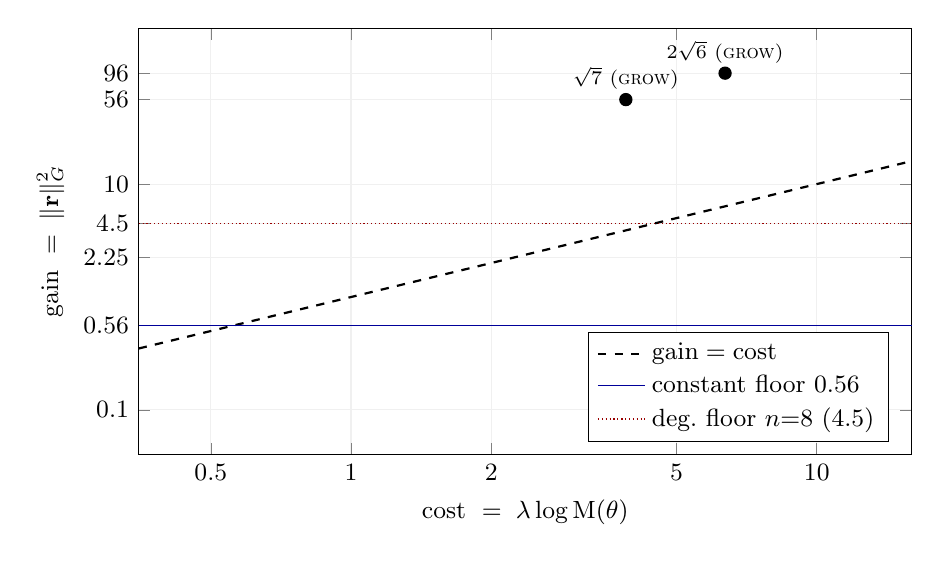
\begin{tikzpicture}
\begin{axis}[
  width=11.4cm, height=7cm, xmode=log, ymode=log,
  xlabel={cost $\;=\;\lambda\log\Mah(\theta)$}, ylabel={gain $\;=\;\lVert\rr\rVert_{\GG}^2$},
  xmin=0.35, xmax=16, ymin=0.04, ymax=240,
  xtick={0.5,1,2,5,10}, xticklabels={0.5,1,2,5,10},
  ytick={0.1,0.562,2.25,4.5,10,56,96}, yticklabels={0.1,0.56,2.25,4.5,10,56,96},
  legend pos=south east, legend cell align=left, font=\small,
  grid=both, grid style={gray!12}]
  \addplot[domain=0.35:16, samples=2, thick, dashed] {x}; \addlegendentry{$\mathrm{gain}=\mathrm{cost}$}
  \addplot[domain=0.35:16, samples=2, blue!60!black] {0.562}; \addlegendentry{constant floor $0.56$}
  \addplot[domain=0.35:16, samples=2, red!60!black, densely dotted] {4.5}; \addlegendentry{deg.\ floor $n{=}8$ ($4.5$)}
  \addplot[only marks, mark=*, mark size=2.2pt] coordinates {(6.356,96) (3.892,56)};
  \addplot[only marks, mark=x, mark size=3.2pt, red, thick] coordinates {(6.356,0.1)};
  \node[anchor=south] at (axis cs:6.356,96) {\scriptsize $2\sqrt6$ (\textsc{grow})};
  \node[anchor=south] at (axis cs:3.892,56) {\scriptsize $\sqrt7$ (\textsc{grow})};
  \node[anchor=west] at (axis cs:6.7,0.1) {\scriptsize tiny (\textsc{stop})};
\end{axis}
\end{tikzpicture}
\caption{The growth decision in the $(\text{cost},\text{gain})$ plane (log--log). The shipped cases $2\sqrt6$
($96$ vs $6.356$) and $\sqrt7$ ($56$ vs $3.892$) sit far above both the boundary $\mathrm{gain}=\mathrm{cost}$
and the floors, hence \textsc{grow}; the lattice--aligned tiny residual ($\mathrm{gain}=0.1$) sits below the
constant floor $0.562$ and is \textsc{stop}ped (Example~\ref{ex:noise}). The degree--aware floor is $2.25$ at
$n{=}4$ and $4.5$ at $n{=}8$ (Remark~\ref{rem:degreeaware}). All gain/cost values for the grow cases and the
floors are probe--verified; the tiny--residual mark's horizontal position is illustrative (its decision is the
gain--versus--floor comparison, independent of cost).}
\label{fig:threshold}
\end{figure}

\subsection{A degree--aware floor}
\begin{remark}[Normalising across fields]\label{rem:degreeaware}
Because $\lVert\rr\rVert_{\GG}^2=n\,\Fish_{\mathrm{exp}}(\rr)$ (Theorem~\ref{thm:resfisher}), a \emph{constant}
floor on $\lVert\rr\rVert_{\GG}^2$ corresponds to a Fisher--significance threshold of order $1/n$: in a
high--degree field a residual that is intrinsically tiny still clears a constant floor, because the factor
$n$ inflates the norm. A \emph{degree--aware} floor $n\,\lambda\log\mu_S$ keeps the Fisher--significance
threshold constant across fields. With $\lambda=2$ the degree--aware floor is $2.25$ at $n=4$ and $4.50$ at
$n=8$. A gain of $1$ clears the constant floor $0.562$ but not the degree--aware floor $4.50$ at $n=8$. The
shipped cases ($\mathrm{gain}=96,56$) clear either floor; the degree--aware refinement is for robustness, not
for the present outcomes.
\end{remark}

\subsection{The exact--versus--float boundary, sharpened}
\begin{remark}[The threshold is intrinsically float]\label{rem:thresholdfloat}
The admissibility half of~\eqref{eq:threshold} is exact (Proposition~\ref{prop:cap}). The information half is
not: $\log\Mah(\theta)$ is transcendental, so $\lVert\rr\rVert_{\GG}^2\ge\lambda\log\Mah$ cannot be a pure
$\Q/\Z$ decision. The gain $\lVert\rr\rVert_{\GG}^2$ remains an exact rational; only the cost is real. An
exact gate would therefore require \emph{certified interval arithmetic} on $\log\Mah$ (so that the comparison
becomes a certified rational decision), which we carry out on a representative case below
(Example~\ref{ex:certified}). Thus capacity is exact while the information threshold is, by its nature,
analytic---but still \emph{decidable} with rigor.
\end{remark}

\begin{example}[A certified \textsc{grow} decision]\label{ex:certified}
We perform the certified comparison for $\sqrt7$ (seed $x^2-7$, $\Mah=7$) at $\lambda=2$. Interval arithmetic
yields the rigorous rational enclosure
\[
  \log 7\in[\,1.94591,\ 1.94592\,],\qquad\text{whence}\qquad \lambda\log 7\;\le\; 2\cdot 1.94592=3.89184 .
\]
The gain $\lVert\rr\rVert_{\GG}^2=56$ is an exact rational, and $56\ge 3.89184\ge\lambda\log 7$, so
\textsc{grow} is \emph{certified} with no trust in any rounded value: an exact rational dominates a rigorous
\emph{upper} bound on the cost. The same procedure certifies $2\sqrt6$ (seed $x^2-24$):
$\log 24\in[3.17805,\,3.17806]$ gives $\lambda\log 24\le 6.35612\le 96$. Both enclosures are produced and
checked by the probe (\S\ref{sec:appendix}); a sharper enclosure is needed only when gain and cost fall within
one interval width of each other.
\end{example}

\begin{remark}[The exchange rate is conjectural]\label{rem:exchange}
The rate $\lambda$ is the information price of one parameter. The minimum--description--length principle
\cite{Rissanen} and the Bayesian information criterion \cite{Schwarz} suggest scales of order $1$ to
$\tfrac12\log N$, but the value appropriate to this substrate is not derived here. Likewise the effective
floor constant---Lehmer's $\mu_L$ (conjectural), Smyth's $\mu_S$ (provable, non--reciprocal), or
Dobrowolski's degree--dependent bound---is a modelling choice. These, together with
Conjecture~\ref{conj:model}, are the locus of what remains genuinely open in R1.
\end{remark}

\section{Applications and use cases}\label{sec:apps}

\subsection{Streaming anomaly and novelty detection}
The residual norm is a direct novelty score: $\lVert\rr(\xx)\rVert_{\GG}^2=0$ for in--distribution
(captured) observations and is strictly positive for off--axis novelty. A calibration--gated detector emits
an alert only when (a) the score exceeds threshold and (b) a calibration predicate passes, and surfaces
persistent novelty as a growth \emph{proposal} via Protocol~\ref{prot:growth} without ever auto--acting. The
detector is exact (a float observation is rejected at intake), and it inherits the witness chain: every
surfaced proposal is recorded. By Theorem~\ref{thm:resfisher} the score is, when $1\in\col(\BB)$, a
degree--scaled Fisher information distance---so ``how anomalous'' has an information--geometric meaning, not
merely a Euclidean one.

\begin{example}[A calibration--gated detection]\label{ex:anomaly}
Take the learner of \S\ref{sec:episode} as the in--distribution model: observations in
$\col(\BB)=\Q\oplus\Q\theta$ score $\lVert\rr\rVert_{\GG}^2=0$ and raise no alert. Inject the off--axis
$2\sqrt6$ (score $96$). While the calibration predicate is closed, the detector records the novelty but
\emph{suppresses} the alert; once calibration passes, the same observation raises an alert and surfaces the
growth proposal $x^2-24$---never auto--confirmed. The basis is unchanged until an explicit confirm, and the
surfaced proposal is appended to the witness chain. Thus ``anomalous'' is the exact, calibration--gated event
$\lVert\rr\rVert_{\GG}^2>0$, whose magnitude is an information distance (Theorem~\ref{thm:resfisher}).
\end{example}

\begin{example}[A streaming trace]\label{ex:stream}
Continuing in $\K=\Q(\theta)$, $\theta=\sqrt2+\sqrt3$, with forced basis $\BB=\{1,\theta\}$ and a calibration
predicate that opens after the third observation. Here $2\sqrt6=\theta^2-5\in\col(\BB)^{\perp_{\GG}}$ carries
the off--axis score $96$ (\S\ref{sec:episode}), and ``$1+2\sqrt6$'' has the same residual as $2\sqrt6$ because
its $1$--part already lies in $\col(\BB)$.
\begin{center}
\begin{tabular}{clccl}
\toprule
$t$ & observation & $\lVert\rr\rVert_{\GG}^2$ & calibrated & action \\
\midrule
$1$ & $2-\theta$\ \ (in $\col\BB$)   & $0$  & no  & --- \\
$2$ & $3+4\theta$\ \ (in $\col\BB$)  & $0$  & no  & --- \\
$3$ & $1+2\sqrt6$\ \ (off--axis)     & $96$ & no  & novelty recorded, alert \emph{suppressed} \\
$4$ & $1+2\sqrt6$                    & $96$ & yes & alert; \emph{propose} seed $x^2-24$ \\
$5$ & confirm                        & ---  & yes & basis grows to $\{1,\theta,2\sqrt6\}$; witnessed \\
$6$ & $1+2\sqrt6$                    & $0$  & yes & captured \\
\bottomrule
\end{tabular}
\end{center}
The score is an exact rational at every step; the basis is mutated only at $t=5$, and only by an explicit
confirm. Steps $3$ and $4$ show the calibration gate decoupling \emph{detection} (score $>0$) from
\emph{alerting}, and step $6$ shows capture collapsing the score to $0$ once the seed is adjoined.
\end{example}

\subsection{A capacity--bounded dictionary learner}
Protocol~\ref{prot:growth} with the gate of \S\ref{sec:capacity} is an online dictionary learner whose
capacity is bounded \emph{by arithmetic}, not by a hyperparameter: by Proposition~\ref{prop:cap} only finitely
many seeds are admissible under a fixed budget, so the model cannot silently inflate. Persistence guards
against noise (a residual that averages to zero proposes nothing); the height gate guards against complexity;
the compositum mechanism (\S\ref{subsec:compositum}) extends the same discipline across fields.

\subsection{Computational aspects}\label{subsec:complexity}
Every operation is exact rational (or integer) arithmetic, trading floating speed for reproducibility; we
record the costs. Forming $\GG$ from a basis is $O(n^3)$ rational multiplications, or $O(n^2)$ trace
evaluations given a multiplication table. The projector solve
$P=\BB(\BB\transpose\GG\BB)\inv\BB\transpose\GG$ is an $O(n^3)$ exact linear solve; in streaming use one
appends a column to $\BB$ and updates the small factorisation of $\BB\transpose\GG\BB$ rather than
refactoring. The coordinates--to--minimal--polynomial bridge (Theorem~\ref{thm:bridge}) is a Smith normal
form of the $n\times n$ matrix $xI-\rho(\alpha)$ over $\Q[x]$; with fraction--free (Bareiss--style)
elimination the intermediate coefficients stay controlled and the cost is polynomial in $n$ and the bit--size
of $\alpha$'s coordinates. The admissibility gate is $O(n)$ integer comparisons
(Proposition~\ref{prop:cap}). The only inexact step is the threshold comparison
$\lVert\rr\rVert_{\GG}^2\ge\lambda\log\Mah(\theta)$, evaluated by certified interval arithmetic on
$\log\Mah$ (\S\ref{sec:threshold}) while the gain side stays an exact rational. The standing practical caveat
is rational coefficient growth: exact Gram and projector entries can acquire large numerators and
denominators, so an implementation bounds the working degree and height (which the capacity gate already
enforces) or tests equalities modulo a prime and lifts. None of this alters a decision---it only prices
exactness.

\subsection{Natural gradient and model selection}
Theorem~\ref{thm:gaussfisher} says the trace form is a Fisher metric; consequently moving in the
$\GG$--geometry is a \emph{natural--gradient} step in the sense of Amari \cite{Amari,AmariNagaoka}, not an
ad hoc Euclidean one. The growth rule~\eqref{eq:threshold} is a model--selection criterion in the MDL/BIC
family \cite{Rissanen,Schwarz}: adjoining a parameter (a basis direction) is justified exactly when the
information it explains, $\lVert\rr\rVert_{\GG}^2$, exceeds its description length $\lambda\log\Mah(\theta)$.
The Lehmer floor (Theorem~\ref{thm:smythfloor}, Conjecture~\ref{conj:lehmer}) gives this description length a
strictly positive minimum---an arithmetic Occam bound.

\subsection{The trace form as an exact integer kernel}\label{subsec:kernel}
The trace pairing makes $\K$ a reproducing structure in the sense of kernel methods---but exactly and over
$\Z$. The Minkowski embedding $\sigma$ is a \emph{feature map} $\K\to\R^n$, and the trace form is its kernel,
\[
  T(x,y)=\Tr(xy)=\langle\sigma(x),\sigma(y)\rangle=\sum_k\sigma_k(x)\sigma_k(y),
\]
positive definite on totally real fields and integer--valued on $\OK$. The forced subspace $\col\BB$ is the
span of the chosen ``support vectors''; the projector $P$ is the kernel projection onto them; and
$\lVert\rr\rVert_{\GG}^2$ is the squared kernel distance to that span. Three properties separate this from an
analytic kernel: it is \emph{exact} (decisions over $\Q$, not floating Gram inversions); it is
\emph{integer--valued} on the ring of integers, so its Gram is a lattice Gram with $\det=d_\K$; and it
\emph{carries arithmetic}---the same kernel fixes the discriminant (Proposition~\ref{prop:discvol}), the
different (\S\ref{subsec:dual}), and the height floor (\S\ref{sec:threshold}) that an inner product alone does
not see. Learning is kernelised dictionary growth in which the kernel is a number field.

\subsection{Persistence as exact re--derivation}\label{subsec:persist}
A trained model is, in its entirety, a short list of monic--integer minimal polynomials---the forced
anchors---together with the residual deltas accumulated since the last anchor. Because the geometry is exact,
a restart is \emph{re--derivation}, not deserialisation: from the anchor polynomials one recomputes the
integral basis, the trace--form Gram $\GG$, and the projector $P$ bit--for--bit
(Theorems~\ref{thm:GMM}, \ref{prop:proj}), then replays the deltas. Two consequences are mathematical, not
engineering. First, the reconstructed $\GG$ and $P$ are \emph{identical} to the originals, so a model and its
restart agree as operators, not merely to within a tolerance---there is no approximation to drift. Second,
the stored state is a self--certificate: the witness chain of Protocol~\ref{prot:growth} makes the whole
learning history replayable and tamper--evident, since each growth step is reproducible from its seed by
exact arithmetic. This is the precise sense in which the substrate is exact ``all the way down''---the
persisted object is not an opaque parameter blob but arithmetic that regenerates itself.

\subsection{Toward a live, additive deployment}
The learner is intended to be wired into a host service additively: read--only \emph{observe} and
\emph{propose} endpoints, a single calibration--gated \emph{confirm}, and a persistence model that stores a
model as forced anchors (the seed minimal polynomials) plus residual deltas, so that restart is exact
re--derivation rather than blob reload. We mention this to indicate the intended scope; it is engineering,
not mathematics, and is out of scope for the present paper.

\section{Open problems}\label{sec:open}

\begin{enumerate}[label=(O\arabic*),leftmargin=*]
  \item \textbf{The canonical model (Conjecture~\ref{conj:model}; partially answered in the companion).}
        Is there a principled reason to prefer $c=1$ (Gaussian) or $c=n$ (max--entropy on conjugates)? The
        companion paper supplies a third, framework--native reading---the scale of the self--action eigenframe
        at a critical point of the ladder $x^2+x=C$, namely $c=\sqrt{1+4C}/(2C)$ (golden gate $c=\sqrt5/2$)---and
        shows the exchange rate is then the identity $\lambda=2c$. By Conjecture~\ref{conj:model} (\v{C}encov)
        this remains a principled \emph{choice} of scale, not a derivation: it names a preferred $c$ without
        removing the irreducible freedom the conjecture identifies.
  \item \textbf{Complex embeddings (partially resolved, \S\ref{subsec:complex}).} The Hermitian form
        $G_2=M^{*}M$ treats $r_2>0$ in principle, and the Fisher identities transfer to it
        (Remark~\ref{rem:fishercaveats}). What remains is an exact, probe--level verification on a field with
        $r_2>0$ and confirmation that the max--entropy ($c=n$) model transfers cleanly when the conjugates
        are genuinely complex.
  \item \textbf{The exchange rate $\lambda$.} Derive (rather than posit) the information price of a basis
        direction for this substrate (Remark~\ref{rem:exchange}).
  \item \textbf{The non--disjoint compositum (Remark~\ref{rem:nondisjoint}).} Construct the true compositum
        Gram when the generator's minimal polynomial factors over $\K$ (via a primitive element, resultants,
        and factorisation over a number field).
  \item \textbf{Applying the degree--aware Lehmer floor.} Replace the shipped floor $0$ by the
        information floor of \S\ref{sec:threshold}, computing $\log\Mah$ by certified interval arithmetic and
        conditioning the gate on $1\in\col(\BB)$ (Remark~\ref{rem:degreeaware}).
\end{enumerate}

\begin{remark}[Scope and limitations]\label{rem:limits}
We restate the boundary of what is claimed. The exact layer---membership, the residual, the projector, the
coordinates--to--minimal--polynomial bridge, and admissibility---is decided over $\Q$ and $\Z$ and is proved
or machine--verified. The \emph{thresholding} layer is not exact: $\log\Mah(\theta)$ is transcendental, the
exchange rate $\lambda$ is posited rather than derived, and---crucially---the cost floor is provably positive
only for \emph{non--reciprocal} seeds (Smyth); for reciprocal seeds, such as Salem numbers and units, no
uniform positive floor is known (Remark~\ref{rem:reciprocal}; Lehmer's conjecture). The information--geometry
reading is conformal with a model--dependent constant ($c=1$ or $c=n$), not a unique identity, and requires
$1\in\col(\BB)$. The compositum construction is proved only in the linearly disjoint case. Finally, the
framework yields \emph{finiteness} of the admissible seed set (Northcott, Proposition~\ref{prop:cap}) but no
convergence--rate or sample--complexity guarantee---how quickly a field is learned from observations is not
bounded here, and is left to future work. None of these gaps touches the exact core; each is flagged where it
arises and collected in \S\ref{sec:open}.
\end{remark}

\appendix
\section{Reproducibility}\label{sec:appendix}

Every numerical claim above is reproduced by a machine--checked probe; the exact symbolic and rational
computations are the evidence for the statements marked as verified.
\begin{itemize}[leftmargin=*]
  \item \textbf{Trace forms, embeddings, Fisher matrices} (Theorems~\ref{thm:GMM},
        \ref{thm:gaussfisher}--\ref{thm:resfisher}; \S\ref{sec:infogeo} table): a symbolic probe builds the
        embedding matrices $M$, verifies $\GG=M\transpose M$, computes
        $\Fish_{\mathrm{exp}}=\tfrac1n(\GG-\tfrac1n tt\transpose)$, and asserts $\GG=n\,\Fish_{\mathrm{exp}}$
        on the trace--zero subspace, including $\lVert\sqrt5\rVert_{\GG}^2=10$ and the
        $1\in\col(\BB)$ both--ways check (Remark~\ref{rem:fishercaveats}).
  \item \textbf{Exact heights and admissibility} (Theorem~\ref{thm:height}, Proposition~\ref{prop:cap},
        Example~\ref{ex:heights}): an integer--only probe checks $\deg$, $\operatorname{ch}$, $\sum c_i^2$,
        the Landau certificate $\Mah^2\le\sum c_i^2$ (cross--checked against the float Mahler), the
        rejection of float inputs, and the Northcott count.
  \item \textbf{The growth threshold} (\S\ref{sec:threshold}, \eqref{eq:threshold}): a probe checks that the
        shipped cases clear $\lVert\rr\rVert_{\GG}^2\ge\lambda\log\Mah$, that the Smyth floor is a positive
        minimum, that a sub--floor residual is stopped by the refined gate but not by floor $0$, and that the
        degree--aware floor differs from the constant floor (the values $0.562$, $2.25$, $4.50$).
  \item \textbf{The coordinates--to--minimal--polynomial bridge} (Theorem~\ref{thm:bridge},
        Example~\ref{ex:bridge}) and the compositum (Proposition~\ref{prop:kron}, Example~\ref{ex:adjoin7})
        are exercised by the learner's own tests, including the $\sqrt7$ growth to
        $\Q(\sqrt2,\sqrt3,\sqrt7)$ with $\GG=\GG_\K\otimes\GG_L$.
  \item \textbf{Spectral, discriminant--volume, certified threshold, catalog, figures}
        (Propositions~\ref{prop:spectral}, \ref{prop:discvol}; Remark~\ref{rem:mahlerspectral};
        Examples~\ref{ex:certified}, \ref{ex:noise}; Table~\ref{tab:catalog}; Figures~\ref{fig:proj},
        \ref{fig:mahler}, \ref{fig:threshold}; probe \texttt{test\_paper\_claims.py}, sympy$+$mpmath): asserts
        $M\rho(x)M\inv=\diag(\sigma_k(x))$ and $\charpoly(\rho(\theta))=m_\theta$; $\det\GG=d_\K$ (or
        $\text{index}^2 d_\K$) and the Jeffreys volumes $\sqrt{|d_\K|}$ for the catalog; $\Nm(\mathfrak d)=|d_\K|$;
        the spectral Mahler values $\Mah(\sqrt2+\sqrt3)=5+2\sqrt6$ and $\Mah(\psi)=\mu_S$; the rigorous
        enclosures $\log7\in[1.94591,1.94592]$, $\log24\in[3.17805,3.17806]$ with the certified \textsc{grow}s;
        and the lattice--aligned--noise decision $\tfrac1{10}<0.562$.
\end{itemize}

\begin{table}[ht]
\centering
\footnotesize
\begin{tabular}{p{0.47\textwidth} l l}
\toprule
Statement & Status & Where \\
\midrule
$\GG=M\transpose M$ (trace form $=$ embedding Gram) & Classical (cited) $+$ probe & Thm~\ref{thm:GMM} \\
$\operatorname{spec}\rho(x)=\{\sigma_k(x)\}$; $M$ diagonalises $\rho$ & Classical (cited) $+$ probe & Prop~\ref{prop:spectral} \\
$\det\GG=d_\K$ (integral basis; $[\OK\!:\!\Lambda]^2 d_\K$ for a sub--order); $\operatorname{covol}=\sqrt{|d_\K|}$ (index$\cdot\sqrt{|d_\K|}$ for a sub--order) & Classical (cited) $+$ probe & Thm~\ref{thm:GMM}, Tab~\ref{tab:catalog} \\
$\Nm(\mathfrak d)=|d_\K|$ \ (different) & Classical (cited) $+$ probe & Tab~\ref{tab:catalog} \\
Discriminant $=$ Jeffreys volume $\sqrt{\det\GG}$ (integral basis) & Synthesis (proved) & Prop~\ref{prop:discvol} \\
$\GG=$ Fisher info of a Gaussian location family ($c=1$) & Classical (cited) $+$ probe & Thm~\ref{thm:gaussfisher} \\
$\lVert\rr\rVert_{\GG}^2=n\,\Fish(\rr)$ on the residual subspace ($c=n$) & This work $+$ probe & Thm~\ref{thm:resfisher} \\
$\Mah(\theta)=\prod_{|\lambda|>1}|\lambda|$ (spectral) & Classical (cited) $+$ probe & Rem~\ref{rem:mahlerspectral} \\
$\log\Mah=$ toral topological entropy & Classical (cited) & Prop~\ref{prop:lsw} \\
Smyth floor $\mu_S=1.3247$ (\emph{non--reciprocal only}) & Cited (theorem) & Thm~\ref{thm:smythfloor} \\
Reciprocal--seed floor (Salem numbers, units) & Open (no uniform floor) & Rem~\ref{rem:reciprocal} \\
Certified \textsc{grow} ($\sqrt7$, $2\sqrt6$) via interval $\log\Mah$ & Verified (interval) & Ex~\ref{ex:certified} \\
Compositum $\GG=\GG_\K\otimes\GG_L$ (disjoint) & This work (proved) & Prop~\ref{prop:kron} \\
Bridge $m_\alpha=$ largest invariant factor of $xI-\rho(\alpha)$ & This work (proved) & Thm~\ref{thm:bridge} \\
Canonical statistical model ($c$; \v{C}encov: free up to scale) & Conjectural; named $c\in\{1,n,\sqrt{1+4C}/(2C)\}$ & Conj~\ref{conj:model} \\
Exchange rate $\lambda=2c$ (identity; see companion) & Model--dependent through $c$ only & Rem~\ref{rem:exchange} \\
Lehmer floor $\mu_L=1.176$ & Conjectural & Conj~\ref{conj:lehmer} \\
Non--disjoint compositum Gram & Open & Rem~\ref{rem:nondisjoint} \\
Fisher identities for $r_2>0$ & Open (probe--level) & Rem~\ref{rem:fishercaveats} \\
\bottomrule
\end{tabular}
\caption{Honesty ledger. \emph{Classical (cited)}: a standard result we use and re--verify by probe, not a
contribution of this paper. \emph{This work}/\emph{Synthesis}: assembled or proved here---the Fisher reading,
the residual identity, the discriminant--as--volume framing, and the bridge/compositum constructions.
\emph{Verified (interval)}: a certified rational decision. \emph{Cited (theorem)}: Smyth's floor,
unconditional only for \emph{non--reciprocal} seeds. \emph{Conjectural}/\emph{model--dependent}/\emph{Open}:
the genuinely unsettled parts. Every ``$+$ probe'' row is reproduced by a machine--checked computation
(\S\ref{sec:appendix}).}
\label{tab:ledger}
\end{table}

\paragraph{Provenance.} The information--geometry results (this paper's \S\ref{sec:infogeo}) and the
threshold derivation (\S\ref{sec:threshold}) correspond to verification probes committed at
\texttt{d526098} (Fisher) and \texttt{c5605d7} (threshold); the exact arithmetic core, the height/capacity
gate, the bridge, and the compositum were committed earlier in the same line of work. The expansion's new
numbers---the figures, the spectral and discriminant--volume results, the certified--interval decisions, and
the fields catalog---are reproduced by the additive probe \texttt{test\_paper\_claims.py} (sympy and mpmath).
All numerical values displayed here match those probes.

\begin{thebibliography}{99}
\bibitem{Northcott} D.~G.~Northcott, \emph{An inequality in the theory of arithmetic on algebraic
  varieties}, Proc. Cambridge Philos. Soc. \textbf{45} (1949), 502--509.
\bibitem{Lehmer} D.~H.~Lehmer, \emph{Factorization of certain cyclotomic functions}, Ann. of Math.
  \textbf{34} (1933), 461--479.
\bibitem{Smyth} C.~J.~Smyth, \emph{On the product of the conjugates outside the unit circle of an algebraic
  integer}, Bull. London Math. Soc. \textbf{3} (1971), 169--175.
\bibitem{Dobrowolski} E.~Dobrowolski, \emph{On a question of Lehmer and the number of irreducible factors of
  a polynomial}, Acta Arith. \textbf{34} (1979), 391--401.
\bibitem{Mahler} K.~Mahler, \emph{An application of Jensen's formula to polynomials}, Mathematika
  \textbf{7} (1960), 98--100.
\bibitem{Landau} E.~Landau, \emph{Sur quelques th\'eor\`emes de M. Petrovitch relatifs aux z\'eros des
  fonctions analytiques}, Bull. Soc. Math. France \textbf{33} (1905), 251--261.
\bibitem{LSW} D.~Lind, K.~Schmidt, T.~Ward, \emph{Mahler measure and entropy for commuting automorphisms of
  compact groups}, Invent. Math. \textbf{101} (1990), 593--629.
\bibitem{BombieriGubler} E.~Bombieri, W.~Gubler, \emph{Heights in Diophantine Geometry}, Cambridge
  University Press, 2006.
\bibitem{Neukirch} J.~Neukirch, \emph{Algebraic Number Theory}, Grundlehren der mathematischen
  Wissenschaften \textbf{322}, Springer, 1999.
\bibitem{Marcus} D.~A.~Marcus, \emph{Number Fields}, Springer, 1977.
\bibitem{DummitFoote} D.~S.~Dummit, R.~M.~Foote, \emph{Abstract Algebra}, 3rd ed., Wiley, 2004.
\bibitem{Amari} S.~Amari, \emph{Information Geometry and Its Applications}, Applied Mathematical Sciences
  \textbf{194}, Springer, 2016.
\bibitem{AmariNagaoka} S.~Amari, H.~Nagaoka, \emph{Methods of Information Geometry}, Translations of
  Mathematical Monographs \textbf{191}, AMS, 2000.
\bibitem{Rissanen} J.~Rissanen, \emph{Modeling by shortest data description}, Automatica \textbf{14}
  (1978), 465--471.
\bibitem{Schwarz} G.~Schwarz, \emph{Estimating the dimension of a model}, Ann. Statist. \textbf{6} (1978),
  461--464.
\bibitem{Jeffreys} H.~Jeffreys, \emph{An invariant form for the prior probability in estimation problems},
  Proc. Roy. Soc. London Ser. A \textbf{186} (1946), 453--461.
\bibitem{Yuzvinskii} S.~A.~Yuzvinskii, \emph{Metric properties of endomorphisms of compact groups}, Izv.
  Akad. Nauk SSSR Ser. Mat. \textbf{29} (1965), 1295--1328; R.~Bowen, \emph{Entropy for group endomorphisms
  and homogeneous spaces}, Trans. Amer. Math. Soc. \textbf{153} (1971), 401--414.
\bibitem{Bilu} Yu.~Bilu, \emph{Limit distribution of small points on algebraic tori}, Duke Math. J.
  \textbf{89} (1997), 465--476.
\bibitem{Cencov} N.~N.~\v{C}encov, \emph{Statistical Decision Rules and Optimal Inference}, Translations of
  Mathematical Monographs \textbf{53}, AMS, 1982.
\end{thebibliography}

\end{document}
